% Options for packages loaded elsewhere
\PassOptionsToPackage{unicode}{hyperref}
\PassOptionsToPackage{hyphens}{url}
%
\documentclass[
]{article}
\usepackage{lmodern}
\usepackage{amssymb,amsmath}
\usepackage{ifxetex,ifluatex}
\ifnum 0\ifxetex 1\fi\ifluatex 1\fi=0 % if pdftex
  \usepackage[T1]{fontenc}
  \usepackage[utf8]{inputenc}
  \usepackage{textcomp} % provide euro and other symbols
\else % if luatex or xetex
  \usepackage{unicode-math}
  \defaultfontfeatures{Scale=MatchLowercase}
  \defaultfontfeatures[\rmfamily]{Ligatures=TeX,Scale=1}
\fi
% Use upquote if available, for straight quotes in verbatim environments
\IfFileExists{upquote.sty}{\usepackage{upquote}}{}
\IfFileExists{microtype.sty}{% use microtype if available
  \usepackage[]{microtype}
  \UseMicrotypeSet[protrusion]{basicmath} % disable protrusion for tt fonts
}{}
\makeatletter
\@ifundefined{KOMAClassName}{% if non-KOMA class
  \IfFileExists{parskip.sty}{%
    \usepackage{parskip}
  }{% else
    \setlength{\parindent}{0pt}
    \setlength{\parskip}{6pt plus 2pt minus 1pt}}
}{% if KOMA class
  \KOMAoptions{parskip=half}}
\makeatother
\usepackage{xcolor}
\IfFileExists{xurl.sty}{\usepackage{xurl}}{} % add URL line breaks if available
\IfFileExists{bookmark.sty}{\usepackage{bookmark}}{\usepackage{hyperref}}
\hypersetup{
  pdftitle={Project1},
  pdfauthor={Florian Beiser, Yaolin Ge},
  hidelinks,
  pdfcreator={LaTeX via pandoc}}
\urlstyle{same} % disable monospaced font for URLs
\usepackage[margin=1in]{geometry}
\usepackage{color}
\usepackage{fancyvrb}
\newcommand{\VerbBar}{|}
\newcommand{\VERB}{\Verb[commandchars=\\\{\}]}
\DefineVerbatimEnvironment{Highlighting}{Verbatim}{commandchars=\\\{\}}
% Add ',fontsize=\small' for more characters per line
\usepackage{framed}
\definecolor{shadecolor}{RGB}{248,248,248}
\newenvironment{Shaded}{\begin{snugshade}}{\end{snugshade}}
\newcommand{\AlertTok}[1]{\textcolor[rgb]{0.94,0.16,0.16}{#1}}
\newcommand{\AnnotationTok}[1]{\textcolor[rgb]{0.56,0.35,0.01}{\textbf{\textit{#1}}}}
\newcommand{\AttributeTok}[1]{\textcolor[rgb]{0.77,0.63,0.00}{#1}}
\newcommand{\BaseNTok}[1]{\textcolor[rgb]{0.00,0.00,0.81}{#1}}
\newcommand{\BuiltInTok}[1]{#1}
\newcommand{\CharTok}[1]{\textcolor[rgb]{0.31,0.60,0.02}{#1}}
\newcommand{\CommentTok}[1]{\textcolor[rgb]{0.56,0.35,0.01}{\textit{#1}}}
\newcommand{\CommentVarTok}[1]{\textcolor[rgb]{0.56,0.35,0.01}{\textbf{\textit{#1}}}}
\newcommand{\ConstantTok}[1]{\textcolor[rgb]{0.00,0.00,0.00}{#1}}
\newcommand{\ControlFlowTok}[1]{\textcolor[rgb]{0.13,0.29,0.53}{\textbf{#1}}}
\newcommand{\DataTypeTok}[1]{\textcolor[rgb]{0.13,0.29,0.53}{#1}}
\newcommand{\DecValTok}[1]{\textcolor[rgb]{0.00,0.00,0.81}{#1}}
\newcommand{\DocumentationTok}[1]{\textcolor[rgb]{0.56,0.35,0.01}{\textbf{\textit{#1}}}}
\newcommand{\ErrorTok}[1]{\textcolor[rgb]{0.64,0.00,0.00}{\textbf{#1}}}
\newcommand{\ExtensionTok}[1]{#1}
\newcommand{\FloatTok}[1]{\textcolor[rgb]{0.00,0.00,0.81}{#1}}
\newcommand{\FunctionTok}[1]{\textcolor[rgb]{0.00,0.00,0.00}{#1}}
\newcommand{\ImportTok}[1]{#1}
\newcommand{\InformationTok}[1]{\textcolor[rgb]{0.56,0.35,0.01}{\textbf{\textit{#1}}}}
\newcommand{\KeywordTok}[1]{\textcolor[rgb]{0.13,0.29,0.53}{\textbf{#1}}}
\newcommand{\NormalTok}[1]{#1}
\newcommand{\OperatorTok}[1]{\textcolor[rgb]{0.81,0.36,0.00}{\textbf{#1}}}
\newcommand{\OtherTok}[1]{\textcolor[rgb]{0.56,0.35,0.01}{#1}}
\newcommand{\PreprocessorTok}[1]{\textcolor[rgb]{0.56,0.35,0.01}{\textit{#1}}}
\newcommand{\RegionMarkerTok}[1]{#1}
\newcommand{\SpecialCharTok}[1]{\textcolor[rgb]{0.00,0.00,0.00}{#1}}
\newcommand{\SpecialStringTok}[1]{\textcolor[rgb]{0.31,0.60,0.02}{#1}}
\newcommand{\StringTok}[1]{\textcolor[rgb]{0.31,0.60,0.02}{#1}}
\newcommand{\VariableTok}[1]{\textcolor[rgb]{0.00,0.00,0.00}{#1}}
\newcommand{\VerbatimStringTok}[1]{\textcolor[rgb]{0.31,0.60,0.02}{#1}}
\newcommand{\WarningTok}[1]{\textcolor[rgb]{0.56,0.35,0.01}{\textbf{\textit{#1}}}}
\usepackage{graphicx,grffile}
\makeatletter
\def\maxwidth{\ifdim\Gin@nat@width>\linewidth\linewidth\else\Gin@nat@width\fi}
\def\maxheight{\ifdim\Gin@nat@height>\textheight\textheight\else\Gin@nat@height\fi}
\makeatother
% Scale images if necessary, so that they will not overflow the page
% margins by default, and it is still possible to overwrite the defaults
% using explicit options in \includegraphics[width, height, ...]{}
\setkeys{Gin}{width=\maxwidth,height=\maxheight,keepaspectratio}
% Set default figure placement to htbp
\makeatletter
\def\fps@figure{htbp}
\makeatother
\setlength{\emergencystretch}{3em} % prevent overfull lines
\providecommand{\tightlist}{%
  \setlength{\itemsep}{0pt}\setlength{\parskip}{0pt}}
\setcounter{secnumdepth}{-\maxdimen} % remove section numbering

\title{Project1}
\usepackage{etoolbox}
\makeatletter
\providecommand{\subtitle}[1]{% add subtitle to \maketitle
  \apptocmd{\@title}{\par {\large #1 \par}}{}{}
}
\makeatother
\subtitle{Markov Chain Monte Carlo techniques}
\author{Florian Beiser, Yaolin Ge}
\date{}

\begin{document}
\maketitle

\hypertarget{metropolis-hastings-for-bivariate-densities}{%
\section{1 Metropolis-Hastings for Bivariate
Densities}\label{metropolis-hastings-for-bivariate-densities}}

We consider three different bivariate densities. 1. Standard Gaussian
with correlation 2. Multimodal as muixture of three Gaussians 3. volcano
(unnormalized)

\hypertarget{plotting}{%
\subsection{1.1 Plotting}\label{plotting}}

We start the project with the visulaisation of the respective densities
in \([-5,5]\times[-5,5]\). (Whyever R likes to put more white space left
and right of the plots, but the middle areas are still representative.)

\begin{Shaded}
\begin{Highlighting}[]
\CommentTok{# Auxilliary variables for visualisation}
\NormalTok{x=}\KeywordTok{seq}\NormalTok{(}\OperatorTok{-}\DecValTok{5}\NormalTok{,}\DecValTok{5}\NormalTok{,}\DataTypeTok{by=}\FloatTok{0.1}\NormalTok{)}
\NormalTok{y=}\KeywordTok{seq}\NormalTok{(}\OperatorTok{-}\DecValTok{5}\NormalTok{,}\DecValTok{5}\NormalTok{,}\DataTypeTok{by=}\FloatTok{0.1}\NormalTok{)}

\NormalTok{z1 =}\StringTok{ }\KeywordTok{matrix}\NormalTok{(}\DecValTok{0}\NormalTok{, }\DataTypeTok{ncol=}\DecValTok{101}\NormalTok{, }\DataTypeTok{nrow=}\DecValTok{101}\NormalTok{)}
\NormalTok{z2 =}\StringTok{ }\KeywordTok{matrix}\NormalTok{(}\DecValTok{0}\NormalTok{, }\DataTypeTok{ncol=}\DecValTok{101}\NormalTok{, }\DataTypeTok{nrow=}\DecValTok{101}\NormalTok{)}
\NormalTok{z3 =}\StringTok{ }\KeywordTok{matrix}\NormalTok{(}\DecValTok{0}\NormalTok{, }\DataTypeTok{ncol=}\DecValTok{101}\NormalTok{, }\DataTypeTok{nrow=}\DecValTok{101}\NormalTok{)}

\KeywordTok{par}\NormalTok{(}\DataTypeTok{mfrow=}\KeywordTok{c}\NormalTok{(}\DecValTok{1}\NormalTok{,}\DecValTok{3}\NormalTok{))}

\CommentTok{##############################################}
\CommentTok{# 1. Standard Gaussian with Correlation}

\CommentTok{# Parameters}
\NormalTok{Sigma =}\StringTok{ }\KeywordTok{matrix}\NormalTok{(}\KeywordTok{c}\NormalTok{(}\DecValTok{1}\NormalTok{,}\FloatTok{0.9}\NormalTok{,}\FloatTok{0.9}\NormalTok{,}\DecValTok{1}\NormalTok{), }\DataTypeTok{nrow=}\DecValTok{2}\NormalTok{)}
\NormalTok{SigmaInv =}\StringTok{ }\KeywordTok{solve}\NormalTok{(Sigma)}
\NormalTok{SigmaSqrt =}\StringTok{ }\KeywordTok{sqrt}\NormalTok{(}\KeywordTok{det}\NormalTok{(Sigma))}

\CommentTok{# Density}
\NormalTok{myGaussian <-}\StringTok{ }\ControlFlowTok{function}\NormalTok{(x)\{}
\NormalTok{  f =}\StringTok{ }\DecValTok{1}\OperatorTok{/}\NormalTok{(}\DecValTok{2}\OperatorTok{*}\NormalTok{pi}\OperatorTok{*}\NormalTok{SigmaSqrt)}\OperatorTok{*}\KeywordTok{exp}\NormalTok{(}\OperatorTok{-}\FloatTok{0.5}\OperatorTok{*}\KeywordTok{t}\NormalTok{(x)}\OperatorTok\NormalTok{SigmaInv}\OperatorTok\NormalTok{x)}
  \KeywordTok{return}\NormalTok{(f)}
\NormalTok{\}}

\CommentTok{# Fill z }
\ControlFlowTok{for}\NormalTok{ (i }\ControlFlowTok{in} \DecValTok{1}\OperatorTok{:}\DecValTok{101}\NormalTok{)\{}
  \ControlFlowTok{for}\NormalTok{ (j }\ControlFlowTok{in} \DecValTok{1}\OperatorTok{:}\DecValTok{101}\NormalTok{)\{}
\NormalTok{    z1[i,j] =}\StringTok{ }\KeywordTok{myGaussian}\NormalTok{(}\KeywordTok{c}\NormalTok{(x[i],y[j]))}
\NormalTok{  \}}
\NormalTok{\}}

\CommentTok{# Visualise}
\KeywordTok{image}\NormalTok{( }\DataTypeTok{x=}\NormalTok{x, }\DataTypeTok{y=}\NormalTok{y, }\DataTypeTok{z=}\NormalTok{z1,}
       \DataTypeTok{asp=}\DecValTok{1}\NormalTok{, }\DataTypeTok{xlab=}\StringTok{"x"}\NormalTok{, }\DataTypeTok{ylab=}\StringTok{"y"}\NormalTok{,}
       \DataTypeTok{main=}\StringTok{"Analytical Density of Standard Gaussian with Correlation"}\NormalTok{)}


\CommentTok{##############################################}
\CommentTok{# 2. Multimodal}

\CommentTok{# Parameters}
\NormalTok{mu1 =}\StringTok{ }\KeywordTok{c}\NormalTok{(}\OperatorTok{-}\FloatTok{1.5}\NormalTok{,}\OperatorTok{-}\FloatTok{1.5}\NormalTok{)}
\NormalTok{Sigma1 =}\StringTok{ }\KeywordTok{matrix}\NormalTok{(}\KeywordTok{c}\NormalTok{(}\DecValTok{1}\NormalTok{,}\DecValTok{0}\NormalTok{,}\DecValTok{0}\NormalTok{,}\DecValTok{1}\NormalTok{), }\DataTypeTok{ncol=}\DecValTok{2}\NormalTok{)}
\NormalTok{Sigma1Inv =}\StringTok{ }\KeywordTok{solve}\NormalTok{(Sigma1)}
\NormalTok{Sigma1Sqrt =}\StringTok{ }\KeywordTok{sqrt}\NormalTok{(}\KeywordTok{det}\NormalTok{(Sigma1))}

\NormalTok{mu2 =}\StringTok{ }\KeywordTok{c}\NormalTok{(}\FloatTok{1.5}\NormalTok{,}\FloatTok{1.5}\NormalTok{)}
\NormalTok{Sigma2 =}\StringTok{ }\KeywordTok{matrix}\NormalTok{(}\KeywordTok{c}\NormalTok{(}\DecValTok{1}\NormalTok{,}\DecValTok{0}\NormalTok{,}\DecValTok{0}\NormalTok{,}\DecValTok{1}\NormalTok{), }\DataTypeTok{ncol=}\DecValTok{2}\NormalTok{)}
\NormalTok{Sigma2Inv =}\StringTok{ }\KeywordTok{solve}\NormalTok{(Sigma2)}
\NormalTok{Sigma2Sqrt =}\StringTok{ }\KeywordTok{sqrt}\NormalTok{(}\KeywordTok{det}\NormalTok{(Sigma2))}

\NormalTok{mu3 =}\StringTok{ }\KeywordTok{c}\NormalTok{(}\OperatorTok{-}\DecValTok{2}\NormalTok{,}\DecValTok{2}\NormalTok{)}
\NormalTok{Sigma3 =}\StringTok{ }\KeywordTok{matrix}\NormalTok{(}\KeywordTok{c}\NormalTok{(}\FloatTok{0.8}\NormalTok{,}\DecValTok{0}\NormalTok{,}\DecValTok{0}\NormalTok{,}\FloatTok{0.8}\NormalTok{), }\DataTypeTok{ncol=}\DecValTok{2}\NormalTok{)}
\NormalTok{Sigma3Inv =}\StringTok{ }\KeywordTok{solve}\NormalTok{(Sigma3)}
\NormalTok{Sigma3Sqrt =}\StringTok{ }\KeywordTok{sqrt}\NormalTok{(}\KeywordTok{det}\NormalTok{(Sigma3))}

\CommentTok{# Density}
\NormalTok{myMultimodal <-}\StringTok{ }\ControlFlowTok{function}\NormalTok{(x)\{}
\NormalTok{  f =}\StringTok{ }\DecValTok{1}\OperatorTok{/}\DecValTok{3} \OperatorTok{*}\StringTok{ }\DecValTok{1}\OperatorTok{/}\NormalTok{(}\DecValTok{2}\OperatorTok{*}\NormalTok{pi}\OperatorTok{*}\NormalTok{Sigma1Sqrt)}\OperatorTok{*}\KeywordTok{exp}\NormalTok{(}\OperatorTok{-}\FloatTok{0.5}\OperatorTok{*}\KeywordTok{t}\NormalTok{(x}\OperatorTok{-}\NormalTok{mu1)}\OperatorTok\NormalTok{Sigma1Inv}\OperatorTok\NormalTok{(x}\OperatorTok{-}\NormalTok{mu1))}
\NormalTok{  f =}\StringTok{ }\NormalTok{f }\OperatorTok{+}\StringTok{ }\DecValTok{1}\OperatorTok{/}\DecValTok{3} \OperatorTok{*}\StringTok{ }\DecValTok{1}\OperatorTok{/}\NormalTok{(}\DecValTok{2}\OperatorTok{*}\NormalTok{pi}\OperatorTok{*}\NormalTok{Sigma2Sqrt)}\OperatorTok{*}\KeywordTok{exp}\NormalTok{(}\OperatorTok{-}\FloatTok{0.5}\OperatorTok{*}\KeywordTok{t}\NormalTok{(x}\OperatorTok{-}\NormalTok{mu2)}\OperatorTok\NormalTok{Sigma2Inv}\OperatorTok\NormalTok{(x}\OperatorTok{-}\NormalTok{mu2))}
\NormalTok{  f =}\StringTok{ }\NormalTok{f }\OperatorTok{+}\StringTok{ }\DecValTok{1}\OperatorTok{/}\DecValTok{3} \OperatorTok{*}\StringTok{ }\DecValTok{1}\OperatorTok{/}\NormalTok{(}\DecValTok{2}\OperatorTok{*}\NormalTok{pi}\OperatorTok{*}\NormalTok{Sigma3Sqrt)}\OperatorTok{*}\KeywordTok{exp}\NormalTok{(}\OperatorTok{-}\FloatTok{0.5}\OperatorTok{*}\KeywordTok{t}\NormalTok{(x}\OperatorTok{-}\NormalTok{mu3)}\OperatorTok\NormalTok{Sigma3Inv}\OperatorTok\NormalTok{(x}\OperatorTok{-}\NormalTok{mu3))}
  \KeywordTok{return}\NormalTok{(f)}
\NormalTok{\}}

\CommentTok{# Fill z}
\ControlFlowTok{for}\NormalTok{ (i }\ControlFlowTok{in} \DecValTok{1}\OperatorTok{:}\DecValTok{101}\NormalTok{)\{}
  \ControlFlowTok{for}\NormalTok{ (j }\ControlFlowTok{in} \DecValTok{1}\OperatorTok{:}\DecValTok{101}\NormalTok{)\{}
\NormalTok{    z2[i,j] =}\StringTok{ }\KeywordTok{myMultimodal}\NormalTok{(}\KeywordTok{c}\NormalTok{(x[i],y[j]))}
\NormalTok{  \}}
\NormalTok{\}}

\CommentTok{# Visualise}
\KeywordTok{image}\NormalTok{( }\DataTypeTok{x=}\NormalTok{x, }\DataTypeTok{y=}\NormalTok{y, }\DataTypeTok{z=}\NormalTok{z2,}
       \DataTypeTok{asp=}\DecValTok{1}\NormalTok{, }\DataTypeTok{xlab=}\StringTok{"x"}\NormalTok{, }\DataTypeTok{ylab=}\StringTok{"y"}\NormalTok{,}
       \DataTypeTok{main=}\StringTok{"Analytical Density of Multimodal"}\NormalTok{)}


\CommentTok{##############################################}
\CommentTok{# 3. Volcano}

\CommentTok{# Density}
\NormalTok{myVolcano <-}\StringTok{ }\ControlFlowTok{function}\NormalTok{(x)\{}
\NormalTok{  f =}\StringTok{ }\DecValTok{1}\OperatorTok{/}\NormalTok{(}\DecValTok{2}\OperatorTok{*}\NormalTok{pi)}\OperatorTok{*}\KeywordTok{exp}\NormalTok{(}\OperatorTok{-}\FloatTok{0.5}\OperatorTok{*}\KeywordTok{t}\NormalTok{(x)}\OperatorTok\NormalTok{x)}\OperatorTok{*}\NormalTok{(}\KeywordTok{t}\NormalTok{(x)}\OperatorTok\NormalTok{x}\FloatTok{+0.25}\NormalTok{)}
  \KeywordTok{return}\NormalTok{(f)}
\NormalTok{\}}

\CommentTok{# Fill z }
\ControlFlowTok{for}\NormalTok{ (i }\ControlFlowTok{in} \DecValTok{1}\OperatorTok{:}\DecValTok{101}\NormalTok{)\{}
  \ControlFlowTok{for}\NormalTok{ (j }\ControlFlowTok{in} \DecValTok{1}\OperatorTok{:}\DecValTok{101}\NormalTok{)\{}
\NormalTok{    z3[i,j] =}\StringTok{ }\KeywordTok{myVolcano}\NormalTok{(}\KeywordTok{c}\NormalTok{(x[i],y[j]))}
\NormalTok{  \}}
\NormalTok{\}}

\CommentTok{# Visualise}
\KeywordTok{image}\NormalTok{( }\DataTypeTok{x=}\NormalTok{x, }\DataTypeTok{y=}\NormalTok{y, }\DataTypeTok{z=}\NormalTok{z3,}
       \DataTypeTok{asp=}\DecValTok{1}\NormalTok{, }\DataTypeTok{xlab=}\StringTok{"x"}\NormalTok{, }\DataTypeTok{ylab=}\StringTok{"y"}\NormalTok{,}
       \DataTypeTok{main=}\StringTok{"Analystical Density of Volcano"}\NormalTok{)}
\end{Highlighting}
\end{Shaded}

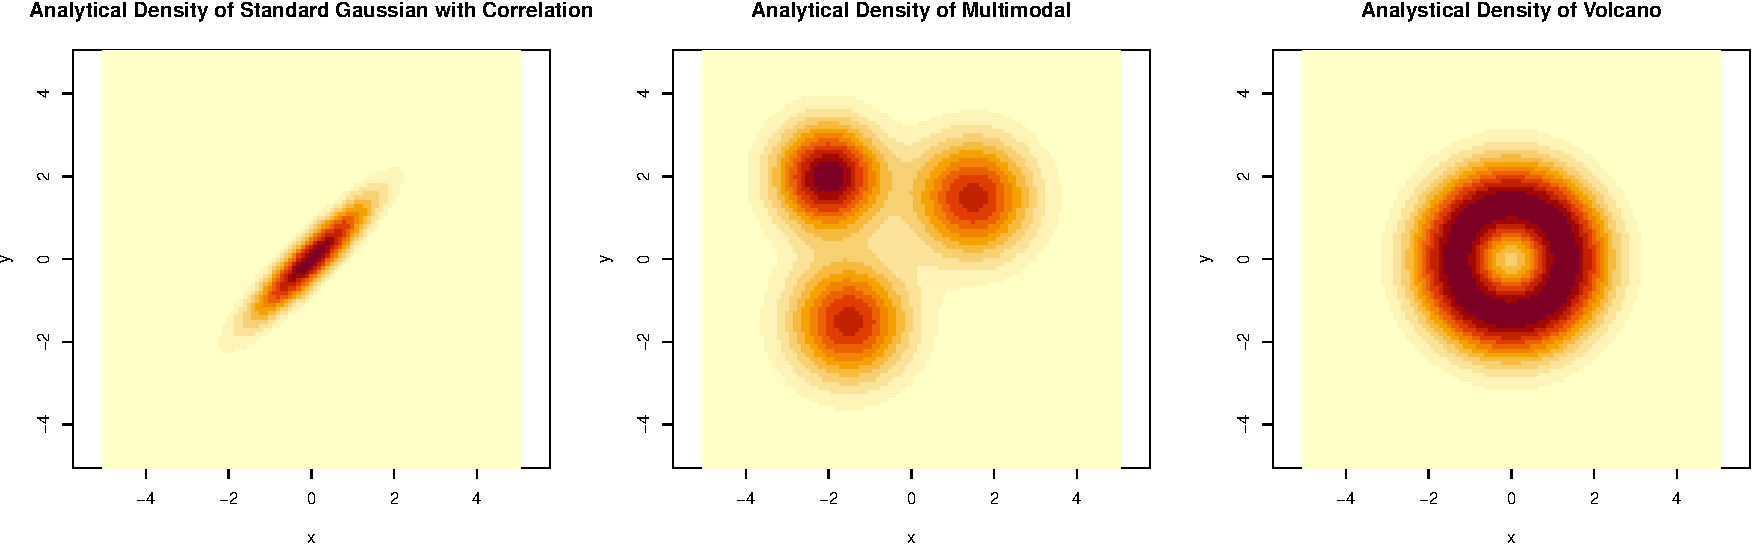
\includegraphics{Project1_files/figure-latex/plotting-1.pdf}

For the subsequent part, where different Metropolis Hastings MCMC
algorithms will be implemented, we prepare with the skeleton that was
discussed in the exercise class and uploaded. This defines the frame for
all MCMC implementations under consideration which differ in the
\texttt{proposal\_func} and \texttt{acceptance\_func}.

\begin{Shaded}
\begin{Highlighting}[]
\CommentTok{# Arguments:}
\CommentTok{# x0 = vector of length 2 with initial values for x}
\CommentTok{# n = number of MCMC iterations to run}
\CommentTok{# proposal_func = function returning a vector of length 2 which is }
\CommentTok{#                 the new proposal}
\CommentTok{# accept_func = function computing the acceptance prob. alpha}
\CommentTok{# dens = function defining your target density}
\NormalTok{mcmc <-}\StringTok{ }\ControlFlowTok{function}\NormalTok{(x0, n, proposal_func, acceptance_func, dens) \{}
  
  \CommentTok{# object to save MCMC samples}
\NormalTok{  x <-}\StringTok{ }\KeywordTok{matrix}\NormalTok{(}\DecValTok{0}\NormalTok{, }\DataTypeTok{nrow=}\NormalTok{n, }\DataTypeTok{ncol=}\DecValTok{2}\NormalTok{)}
\NormalTok{  alphas <-}\StringTok{ }\KeywordTok{rep}\NormalTok{(}\DecValTok{0}\NormalTok{,n)}
  \CommentTok{# initialisation}
\NormalTok{  x_old <-}\StringTok{ }\NormalTok{x0}
  \CommentTok{# generate a vector of n uniform distributed random variables}
\NormalTok{  u <-}\StringTok{ }\KeywordTok{runif}\NormalTok{(n)}
  \CommentTok{# go through n itearations}
  \ControlFlowTok{for}\NormalTok{ (i }\ControlFlowTok{in} \DecValTok{1}\OperatorTok{:}\NormalTok{n) \{}
    \CommentTok{# get a new proposal for x}
\NormalTok{    x_prop <-}\StringTok{ }\KeywordTok{proposal_func}\NormalTok{(x_old)}
    \CommentTok{# compute the acceptance prob alpha}
\NormalTok{    alpha <-}\StringTok{ }\KeywordTok{acceptance_func}\NormalTok{(x_prop, x_old, dens)}
\NormalTok{    alphas[i] =}\StringTok{ }\NormalTok{alpha}
    \CommentTok{# decide wether to accept or reject}
    \ControlFlowTok{if}\NormalTok{ (u[i] }\OperatorTok{<}\StringTok{ }\NormalTok{alpha) \{}
\NormalTok{      x_new <-}\StringTok{ }\NormalTok{x_prop}
\NormalTok{    \} }\ControlFlowTok{else}\NormalTok{ \{}
\NormalTok{      x_new <-}\StringTok{ }\NormalTok{x_old}
\NormalTok{    \}}
    \CommentTok{# save the new sample}
\NormalTok{    x[i,] <-}\StringTok{ }\NormalTok{x_new}
\NormalTok{    x_old <-}\StringTok{ }\NormalTok{x_new}
\NormalTok{  \}}
  \KeywordTok{return}\NormalTok{(}\KeywordTok{list}\NormalTok{(}\StringTok{"x"}\NormalTok{=x,}\StringTok{"alphas"}\NormalTok{=alphas))}
\NormalTok{\}}
\end{Highlighting}
\end{Shaded}

These implementation is not tweaked for optimal performance,
e.g.~log-scale could lead to better scaling or reduction of redundant
calculations in the individual MCMC versions could lead to fast
execution, but we want to the same skeleton for all algorithms to
higlight similarities and differences. For the analysis of the outcomes,
we use below's plotting functionality.

\begin{Shaded}
\begin{Highlighting}[]
\CommentTok{# Arguments:}
\CommentTok{# trace = trace of MCMC algo [x_1,x_2]^n}

\CommentTok{# Function:}
\CommentTok{# - Density plots}
\CommentTok{# - Trace plots}
\CommentTok{# - Autocorrelation}
\NormalTok{MCMCplots <-}\StringTok{ }\ControlFlowTok{function}\NormalTok{(trace, }\DataTypeTok{surface=}\OtherTok{FALSE}\NormalTok{)\{}
  \CommentTok{# Generating empirical densitty}
\NormalTok{  kd =}\StringTok{ }\NormalTok{MASS}\OperatorTok{::}\KeywordTok{kde2d}\NormalTok{(}\DataTypeTok{x=}\NormalTok{trace}\OperatorTok{$}\NormalTok{x[,}\DecValTok{1}\NormalTok{], }\DataTypeTok{y=}\NormalTok{trace}\OperatorTok{$}\NormalTok{x[,}\DecValTok{2}\NormalTok{], }\DataTypeTok{n=}\DecValTok{101}\NormalTok{, }\DataTypeTok{lims=}\KeywordTok{c}\NormalTok{(}\OperatorTok{-}\DecValTok{5}\NormalTok{,}\DecValTok{5}\NormalTok{,}\OperatorTok{-}\DecValTok{5}\NormalTok{,}\DecValTok{5}\NormalTok{))}
  
  \CommentTok{# Nice 3D empirical density plots }
  \CommentTok{# }\AlertTok{WARNING}\CommentTok{: VERY SLOW}
  \ControlFlowTok{if}\NormalTok{ (surface}\OperatorTok{==}\OtherTok{TRUE}\NormalTok{)\{}
    \KeywordTok{library}\NormalTok{(plotly)}
    \KeywordTok{plot_ly}\NormalTok{(}\DataTypeTok{x=}\NormalTok{kd}\OperatorTok{$}\NormalTok{x, }\DataTypeTok{y=}\NormalTok{kd}\OperatorTok{$}\NormalTok{y, }\DataTypeTok{z=}\NormalTok{kd}\OperatorTok{$}\NormalTok{z, }\DataTypeTok{type=}\StringTok{"surface"}\NormalTok{)}
\NormalTok{  \}}
  
  \KeywordTok{layout}\NormalTok{(}\KeywordTok{matrix}\NormalTok{(}\KeywordTok{c}\NormalTok{(}\DecValTok{1}\NormalTok{,}\DecValTok{1}\NormalTok{,}\DecValTok{2}\NormalTok{,}\DecValTok{3}\NormalTok{,}\DecValTok{4}\NormalTok{,}\DecValTok{5}\NormalTok{), }\DecValTok{2}\NormalTok{, }\DecValTok{3}\NormalTok{))}
  
  \CommentTok{# 2D empirical density plots}
  \KeywordTok{image}\NormalTok{( }\DataTypeTok{x=}\NormalTok{kd}\OperatorTok{$}\NormalTok{x, }\DataTypeTok{y=}\NormalTok{kd}\OperatorTok{$}\NormalTok{y, }\DataTypeTok{z=}\NormalTok{kd}\OperatorTok{$}\NormalTok{z,}
         \DataTypeTok{asp=}\DecValTok{1}\NormalTok{, }\DataTypeTok{main=}\StringTok{"Density"}\NormalTok{,}
         \DataTypeTok{xlab=}\StringTok{"x"}\NormalTok{, }\DataTypeTok{ylab=}\StringTok{"y"}\NormalTok{, }\DataTypeTok{xlim=}\KeywordTok{c}\NormalTok{(}\OperatorTok{-}\DecValTok{5}\NormalTok{,}\DecValTok{5}\NormalTok{), }\DataTypeTok{ylim=}\KeywordTok{c}\NormalTok{(}\OperatorTok{-}\DecValTok{5}\NormalTok{,}\DecValTok{5}\NormalTok{))}
  
  \CommentTok{# Trace plots}
  \KeywordTok{plot}\NormalTok{(trace}\OperatorTok{$}\NormalTok{x[,}\DecValTok{1}\NormalTok{], }\DataTypeTok{type=}\StringTok{"l"}\NormalTok{, }\DataTypeTok{ylab=}\StringTok{"x1"}\NormalTok{, }
     \DataTypeTok{main=}\StringTok{"Trace of x1"}\NormalTok{, }\DataTypeTok{ylim=}\KeywordTok{c}\NormalTok{(}\OperatorTok{-}\FloatTok{3.5}\NormalTok{,}\FloatTok{3.5}\NormalTok{))}
  \KeywordTok{plot}\NormalTok{(trace}\OperatorTok{$}\NormalTok{x[,}\DecValTok{2}\NormalTok{], }\DataTypeTok{type=}\StringTok{"l"}\NormalTok{, }\DataTypeTok{ylab=}\StringTok{"x2"}\NormalTok{, }
     \DataTypeTok{main=}\StringTok{"Trace of x2"}\NormalTok{, }\DataTypeTok{ylim=}\KeywordTok{c}\NormalTok{(}\OperatorTok{-}\FloatTok{3.5}\NormalTok{,}\FloatTok{3.5}\NormalTok{))}

  \CommentTok{# Autocorrelation}
  \KeywordTok{acf}\NormalTok{(trace}\OperatorTok{$}\NormalTok{x[,}\DecValTok{1}\NormalTok{], }\DataTypeTok{main=}\StringTok{"Autocorrelation for x1"}\NormalTok{)}
  \KeywordTok{acf}\NormalTok{(trace}\OperatorTok{$}\NormalTok{x[,}\DecValTok{2}\NormalTok{], }\DataTypeTok{main=}\StringTok{"Autocorrelation for x2"}\NormalTok{)}
  
  \KeywordTok{title}\NormalTok{(}\KeywordTok{paste}\NormalTok{(}\StringTok{"Analysis (tuning parameter sigma="}\NormalTok{,sigma,}
               \StringTok{"and mean acceptance rate"}\NormalTok{, }\KeywordTok{sum}\NormalTok{(trace}\OperatorTok{$}\NormalTok{alphas)}\OperatorTok{/}\KeywordTok{length}\NormalTok{(trace}\OperatorTok{$}\NormalTok{alphas),}\StringTok{")"}\NormalTok{), }
        \DataTypeTok{outer=}\OtherTok{TRUE}\NormalTok{)}
\NormalTok{\}}
\end{Highlighting}
\end{Shaded}

We will use the same input parameters for all subsequent MCMC
calculations, the tuning parameters are of course not influenced.

\begin{Shaded}
\begin{Highlighting}[]
\CommentTok{# Input}
\NormalTok{x0 =}\StringTok{ }\KeywordTok{c}\NormalTok{(}\DecValTok{0}\NormalTok{,}\DecValTok{0}\NormalTok{)}
\NormalTok{n =}\StringTok{ }\DecValTok{2000}
\end{Highlighting}
\end{Shaded}

\hypertarget{random-walk-mh}{%
\subsection{1.2 Random walk MH}\label{random-walk-mh}}

The random walk MH uses a symmetric
\(\mathcal{N}(\texttt{x_old},\sigma^2)\) distribution to generate the
new proposal. Moreover, the general MH acceptance probability
simplifies.

\begin{Shaded}
\begin{Highlighting}[]
\CommentTok{# Loads}
\KeywordTok{library}\NormalTok{(mvtnorm)}

\CommentTok{# Arguments: }
\CommentTok{# x_old = old state [x_1_old, x_2_old]}

\CommentTok{# Function:}
\CommentTok{# Generating proposal following the Random walk MH}

\CommentTok{# Return:}
\CommentTok{# x_prop = proposed state [x_1_prop, x_2_prop]}
\NormalTok{RWproposal <-}\StringTok{ }\ControlFlowTok{function}\NormalTok{(x_old)\{}
\NormalTok{  x_prop =}\StringTok{ }\KeywordTok{c}\NormalTok{(}\KeywordTok{rmvnorm}\NormalTok{(}\DecValTok{1}\NormalTok{, x_old, sigma}\OperatorTok{**}\DecValTok{2} \OperatorTok{*}\StringTok{ }\KeywordTok{diag}\NormalTok{(}\DecValTok{1}\NormalTok{,}\DecValTok{2}\NormalTok{,}\DecValTok{2}\NormalTok{)))}
  \KeywordTok{return}\NormalTok{(x_prop)}
\NormalTok{\}}

\CommentTok{# Arguments: }
\CommentTok{# x_prop = proposed state [x_1_prop, x_2_prop]}
\CommentTok{# x_old = old state [x_1_old, x_2_old]}
\CommentTok{# dens = density function of target dist}

\CommentTok{# Function:}
\CommentTok{# Calculating acceptance prob for random walk MH}

\CommentTok{# Return:}
\CommentTok{# alpha = acceptance probability (numeric)}
\NormalTok{RWacceptance <-}\StringTok{ }\ControlFlowTok{function}\NormalTok{(x_prop, x_old, dens)\{}
\NormalTok{  alpha =}\StringTok{ }\KeywordTok{min}\NormalTok{(}\DecValTok{1}\NormalTok{, }\KeywordTok{dens}\NormalTok{(x_prop)}\OperatorTok{/}\KeywordTok{dens}\NormalTok{(x_old))}
  \KeywordTok{return}\NormalTok{(alpha)}
\NormalTok{\}}
\end{Highlighting}
\end{Shaded}

\hypertarget{standard-gaussian}{%
\subsubsection{Standard Gaussian}\label{standard-gaussian}}

We first test the Random Walk MH for the Gaussian with different tuning
parameters \(\sigma\) in the proposal distribution.

\begin{Shaded}
\begin{Highlighting}[]
\CommentTok{##############################}
\CommentTok{# Testing Random Walk for Gaussian}

\CommentTok{# Tuning parameters}
\NormalTok{sigma =}\StringTok{ }\FloatTok{0.1}
\NormalTok{trace0 =}\StringTok{ }\KeywordTok{mcmc}\NormalTok{(x0, n, RWproposal, RWacceptance, myGaussian )}
\KeywordTok{MCMCplots}\NormalTok{(trace0)}
\end{Highlighting}
\end{Shaded}

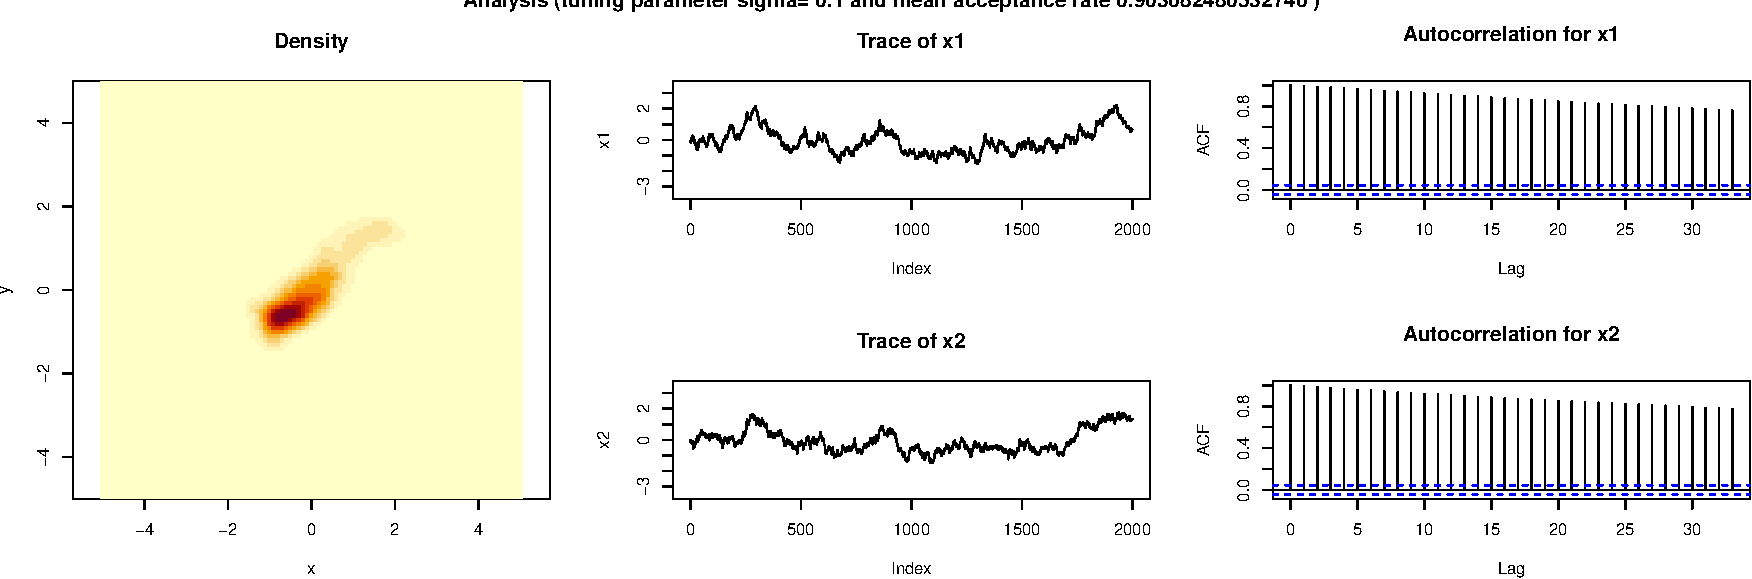
\includegraphics{Project1_files/figure-latex/RandomWalk1-1.pdf}

\begin{Shaded}
\begin{Highlighting}[]
\NormalTok{sigma =}\StringTok{ }\FloatTok{0.5} 
\NormalTok{trace1 =}\StringTok{ }\KeywordTok{mcmc}\NormalTok{(x0, n, RWproposal, RWacceptance, myGaussian )}
\KeywordTok{MCMCplots}\NormalTok{(trace1)}
\end{Highlighting}
\end{Shaded}

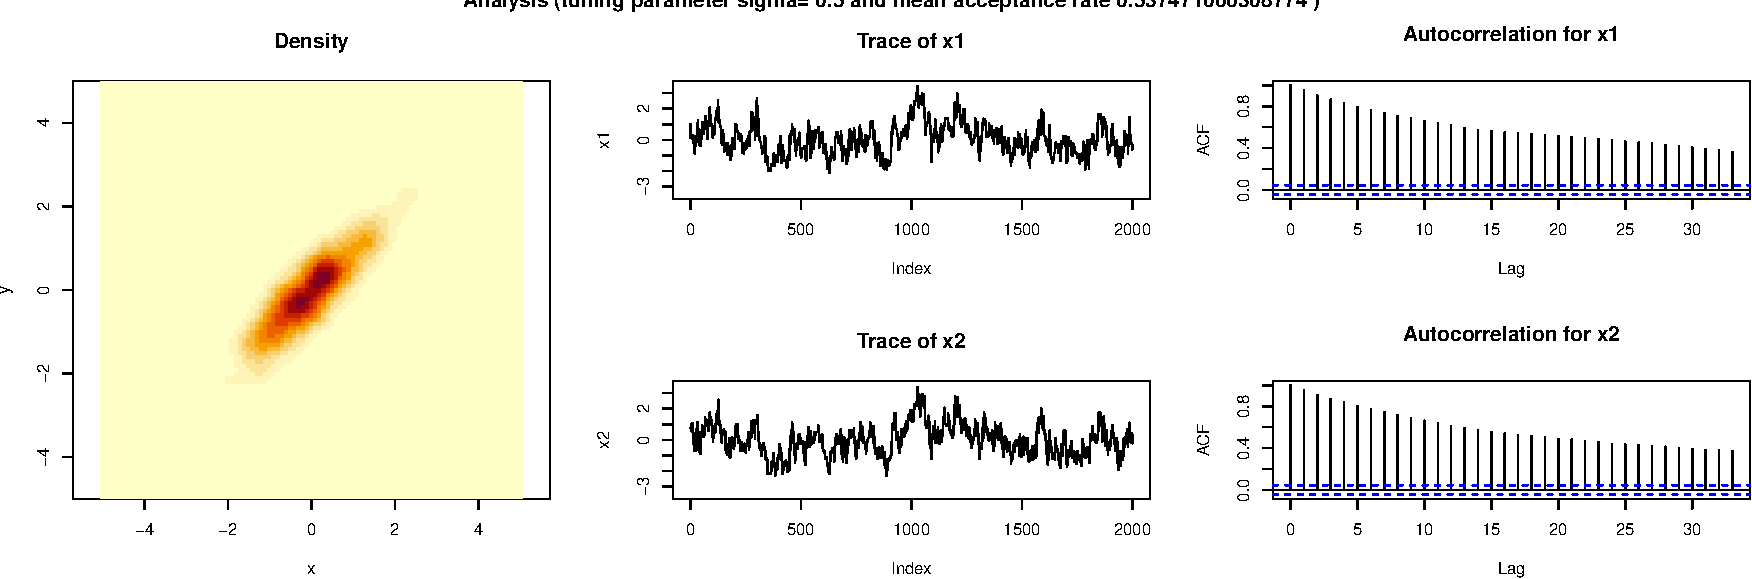
\includegraphics{Project1_files/figure-latex/RandomWalk1-2.pdf}

\begin{Shaded}
\begin{Highlighting}[]
\NormalTok{sigma =}\StringTok{ }\FloatTok{1.0}
\NormalTok{trace2 =}\StringTok{ }\KeywordTok{mcmc}\NormalTok{(x0, n, RWproposal, RWacceptance, myGaussian )}
\KeywordTok{MCMCplots}\NormalTok{(trace2)}
\end{Highlighting}
\end{Shaded}

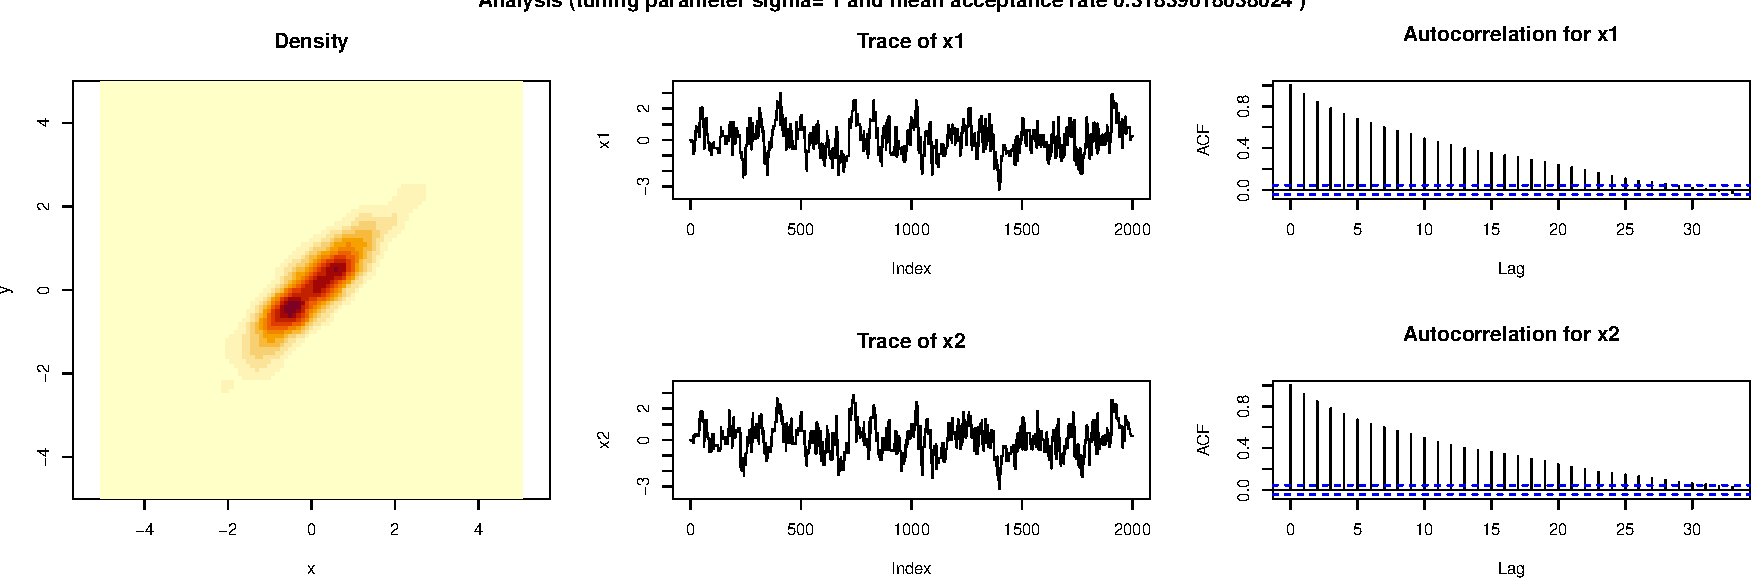
\includegraphics{Project1_files/figure-latex/RandomWalk1-3.pdf}

\begin{Shaded}
\begin{Highlighting}[]
\NormalTok{sigma =}\StringTok{ }\FloatTok{2.5}
\NormalTok{trace3 =}\StringTok{ }\KeywordTok{mcmc}\NormalTok{(x0, n, RWproposal, RWacceptance, myGaussian )}
\KeywordTok{MCMCplots}\NormalTok{(trace3)}
\end{Highlighting}
\end{Shaded}

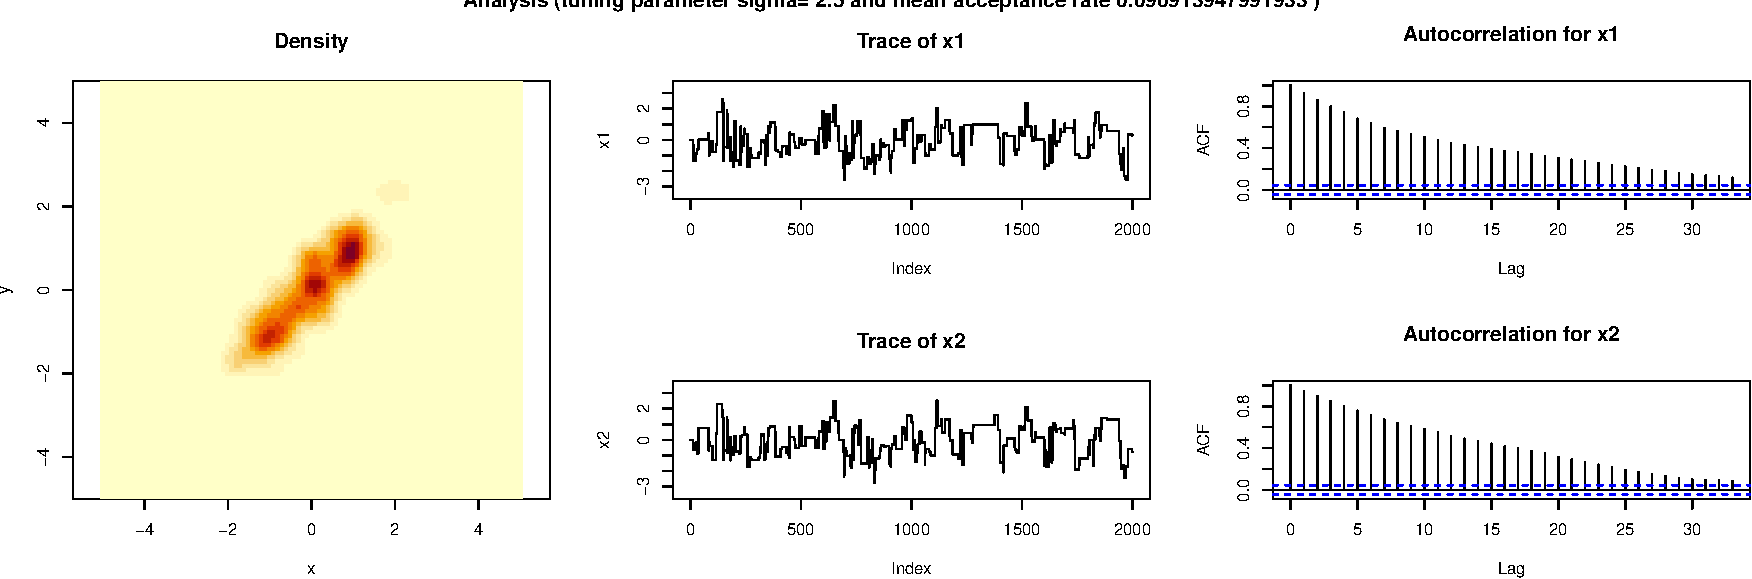
\includegraphics{Project1_files/figure-latex/RandomWalk1-4.pdf}

Depending on the choice of the tuning parameter the MCMC algorithms show
different efficiency. Actually all tuning parameters explore the
state-space rather sedately. However, for values \(\sigma<0.5\) the mean
acceptance rate gets bigger than recommended and the traces change in
too little step, for values \(\sigma>1.5\) the traces start to pause in
a level due to a too small acceptance rate. We recommend values
\(\sigma\in(0.5,1.5)\) for the Gaussian, since for those values the
autocorrelation has t he smallest lag and shrinks at least after 20
steps (what is still much).

\hypertarget{multimodal}{%
\subsubsection{Multimodal}\label{multimodal}}

We continue with application of the Random Walk MH to the Multimodal
with different tuning parameters \(\sigma\) in the proposal
distribution.

\begin{Shaded}
\begin{Highlighting}[]
\CommentTok{##############################}
\CommentTok{# Testing Random Walk for Multimodal}

\CommentTok{# Tuning parameters}
\NormalTok{sigma =}\StringTok{ }\FloatTok{0.1}
\NormalTok{trace1 =}\StringTok{ }\KeywordTok{mcmc}\NormalTok{(x0, n, RWproposal, RWacceptance, myMultimodal )}
\KeywordTok{MCMCplots}\NormalTok{(trace1)}
\end{Highlighting}
\end{Shaded}

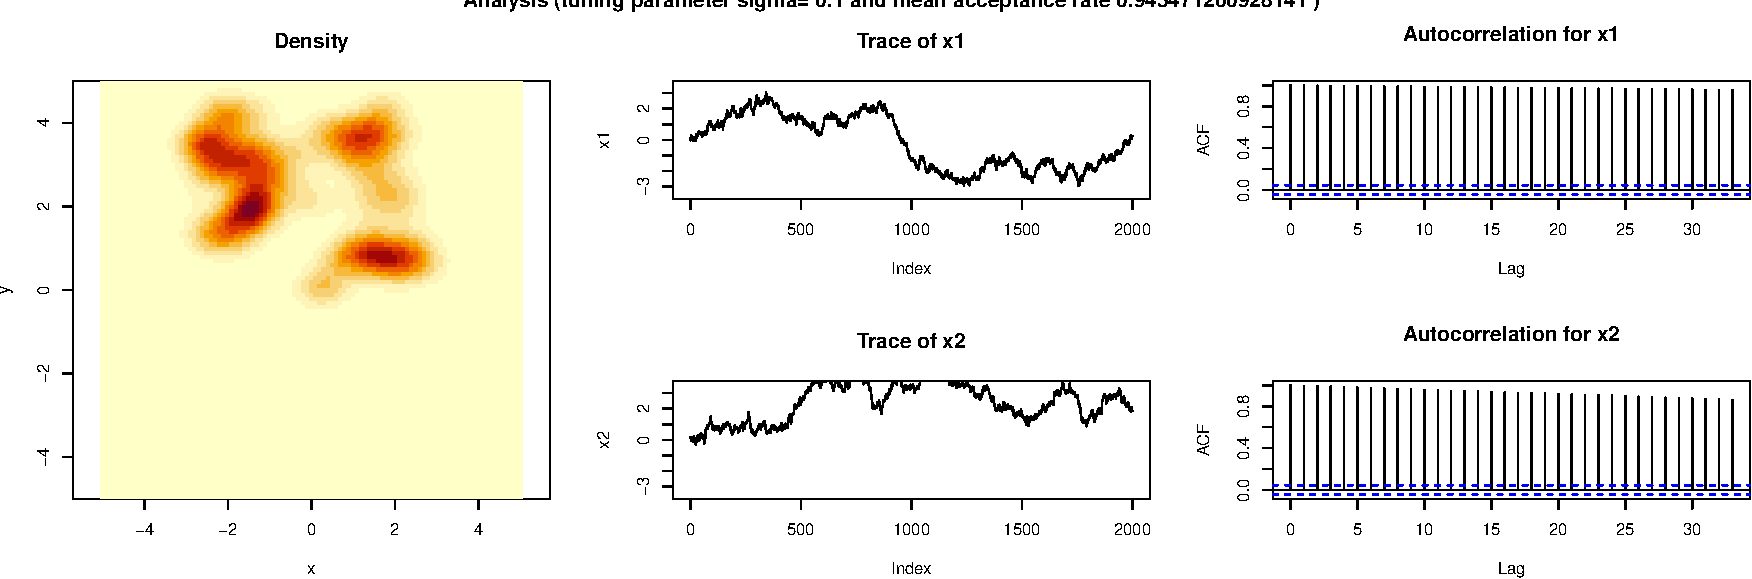
\includegraphics{Project1_files/figure-latex/RandomWalk2-1.pdf}

\begin{Shaded}
\begin{Highlighting}[]
\NormalTok{sigma =}\StringTok{ }\FloatTok{1.0}
\NormalTok{trace2 =}\StringTok{ }\KeywordTok{mcmc}\NormalTok{(x0, n, RWproposal, RWacceptance, myMultimodal )}
\KeywordTok{MCMCplots}\NormalTok{(trace2)}
\end{Highlighting}
\end{Shaded}

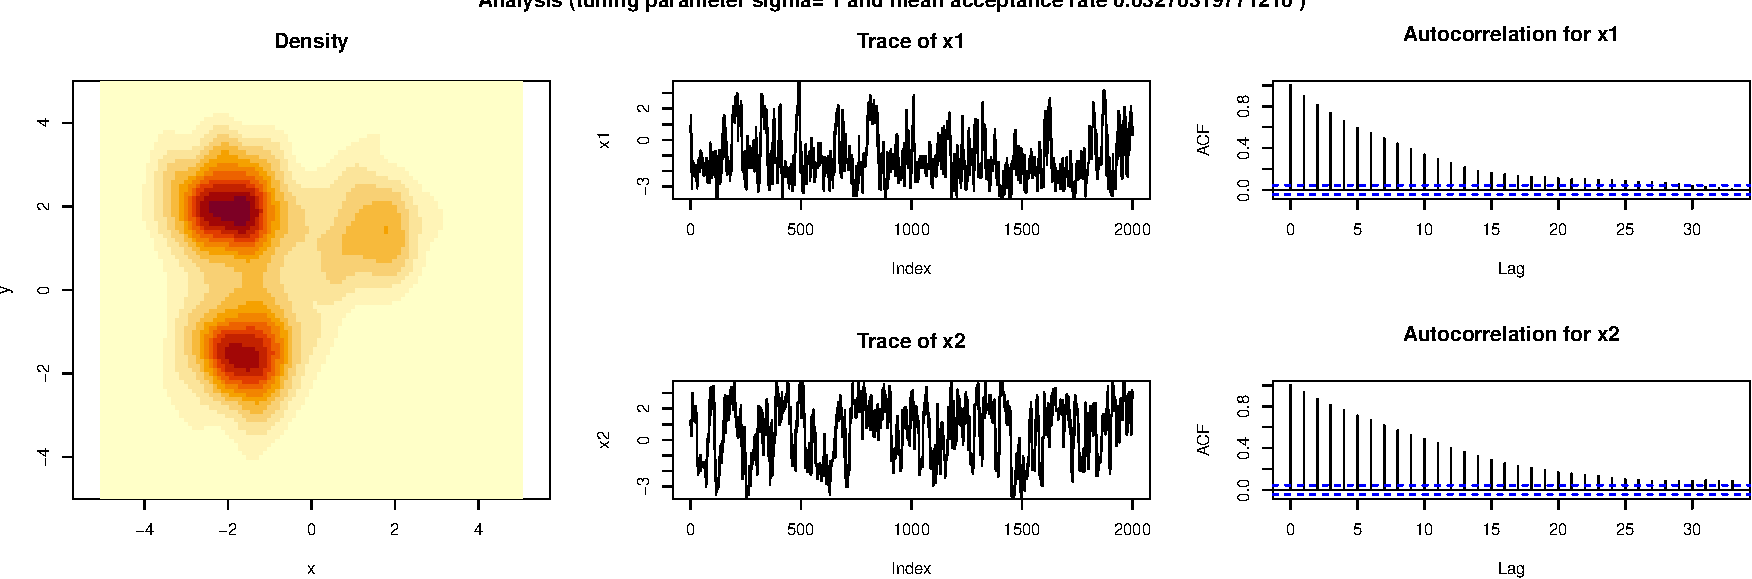
\includegraphics{Project1_files/figure-latex/RandomWalk2-2.pdf}

\begin{Shaded}
\begin{Highlighting}[]
\NormalTok{sigma =}\StringTok{ }\FloatTok{5.0}
\NormalTok{trace3 =}\StringTok{ }\KeywordTok{mcmc}\NormalTok{(x0, n, RWproposal, RWacceptance, myMultimodal )}
\KeywordTok{MCMCplots}\NormalTok{(trace3)}
\end{Highlighting}
\end{Shaded}

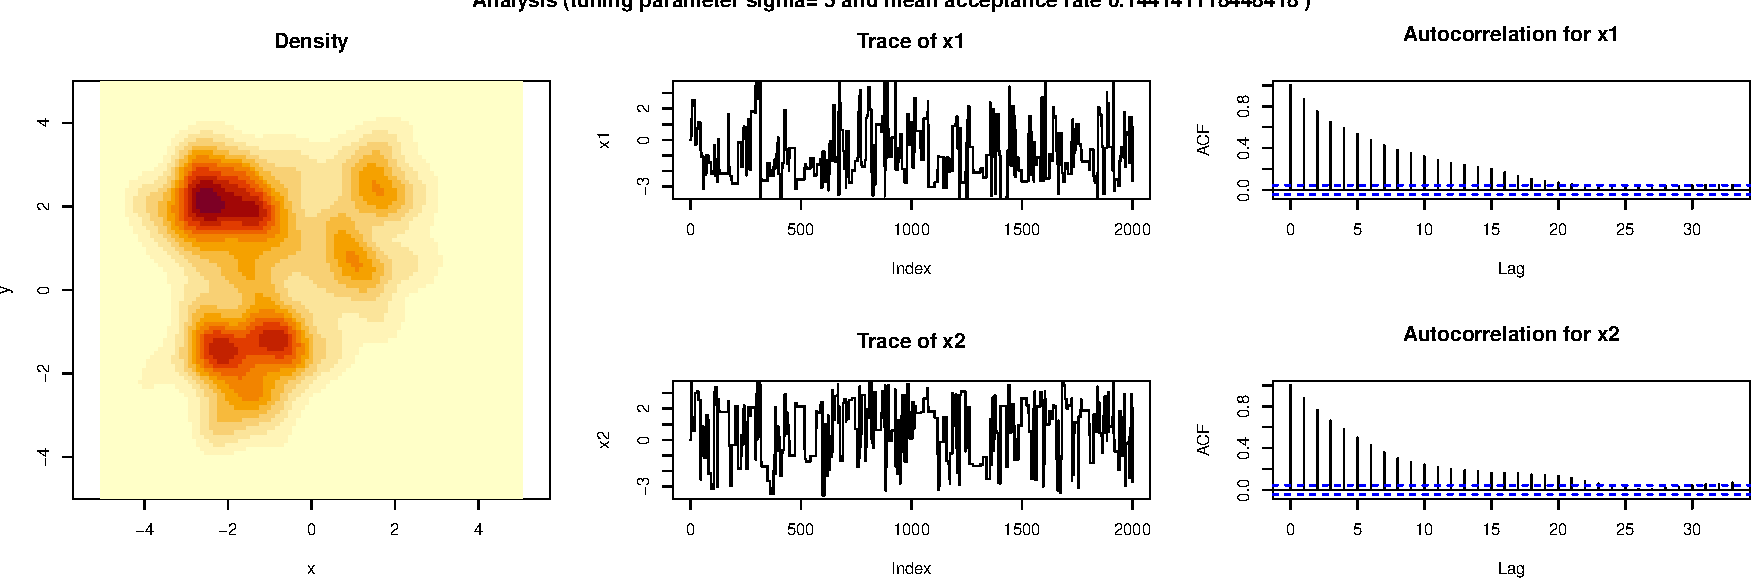
\includegraphics{Project1_files/figure-latex/RandomWalk2-3.pdf}

\begin{Shaded}
\begin{Highlighting}[]
\NormalTok{sigma =}\StringTok{ }\FloatTok{10.0}
\NormalTok{trace3 =}\StringTok{ }\KeywordTok{mcmc}\NormalTok{(x0, n, RWproposal, RWacceptance, myMultimodal )}
\KeywordTok{MCMCplots}\NormalTok{(trace3)}
\end{Highlighting}
\end{Shaded}

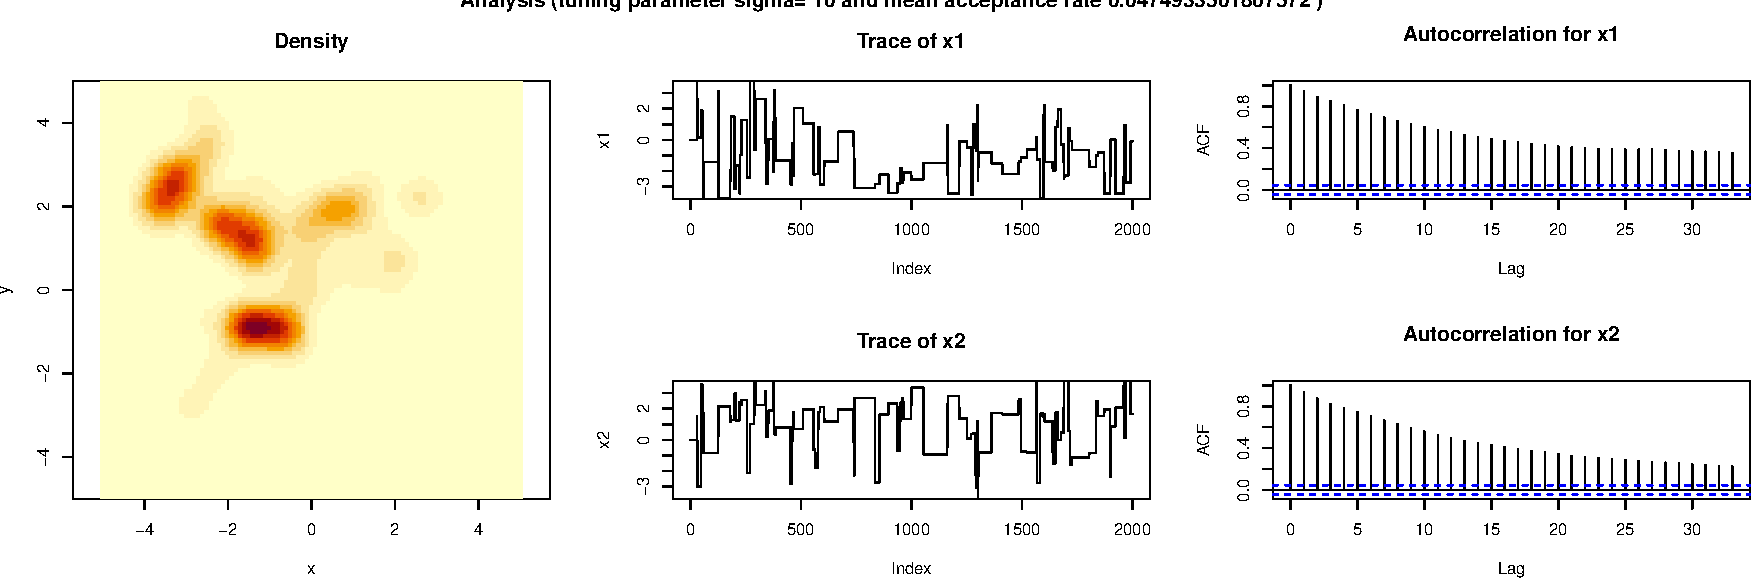
\includegraphics{Project1_files/figure-latex/RandomWalk2-4.pdf}

For the smallest choice of \(\sigma=0.1\) the chain does not really
explore all modes and stays for quite long in one mode when it is there,
therefore the autocorrelation is very high. When increasing up to
\(\sigma=5.0\) we improve the exploration of the different modes and
reduce the autocorrelation significantly. Moreover, the mean acceptance
rate reaches the recommended range. For very high tuning parameter
choices \(\sigma=10.0\), we start to wildly jump from one mode to the
other, but the traces start to pause too long between the jumps.

\hypertarget{volcano}{%
\subsubsection{Volcano}\label{volcano}}

Finally, we try the random walk MH for the volcano shaped density.

\begin{Shaded}
\begin{Highlighting}[]
\CommentTok{##############################}
\CommentTok{# Testing Random Walk for Multimodal}

\CommentTok{# Tuning parameters}
\NormalTok{sigma =}\StringTok{ }\FloatTok{0.1}
\NormalTok{trace1 =}\StringTok{ }\KeywordTok{mcmc}\NormalTok{(x0, n, RWproposal, RWacceptance, myVolcano )}
\KeywordTok{MCMCplots}\NormalTok{(trace1)}
\end{Highlighting}
\end{Shaded}

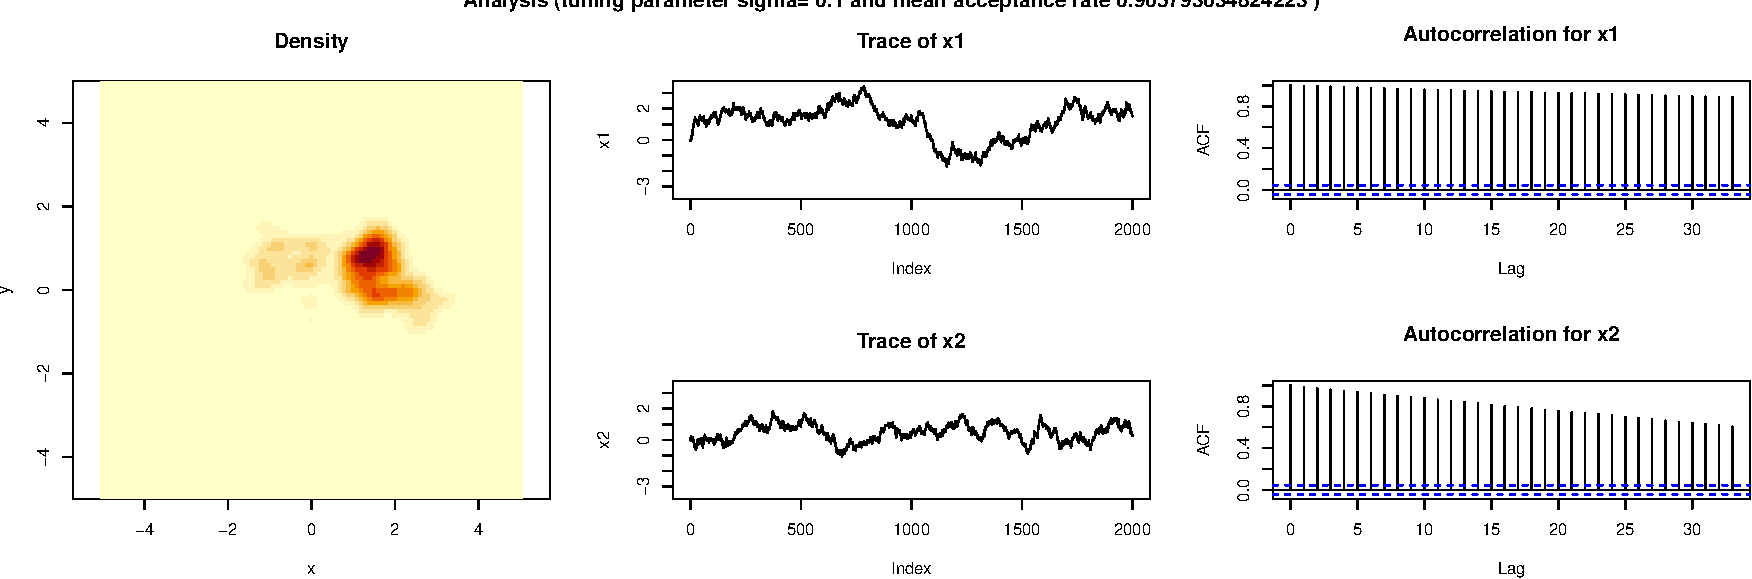
\includegraphics{Project1_files/figure-latex/RandomWalk3-1.pdf}

\begin{Shaded}
\begin{Highlighting}[]
\NormalTok{sigma =}\StringTok{ }\FloatTok{0.5}
\NormalTok{trace2 =}\StringTok{ }\KeywordTok{mcmc}\NormalTok{(x0, n, RWproposal, RWacceptance, myVolcano )}
\KeywordTok{MCMCplots}\NormalTok{(trace2)}
\end{Highlighting}
\end{Shaded}

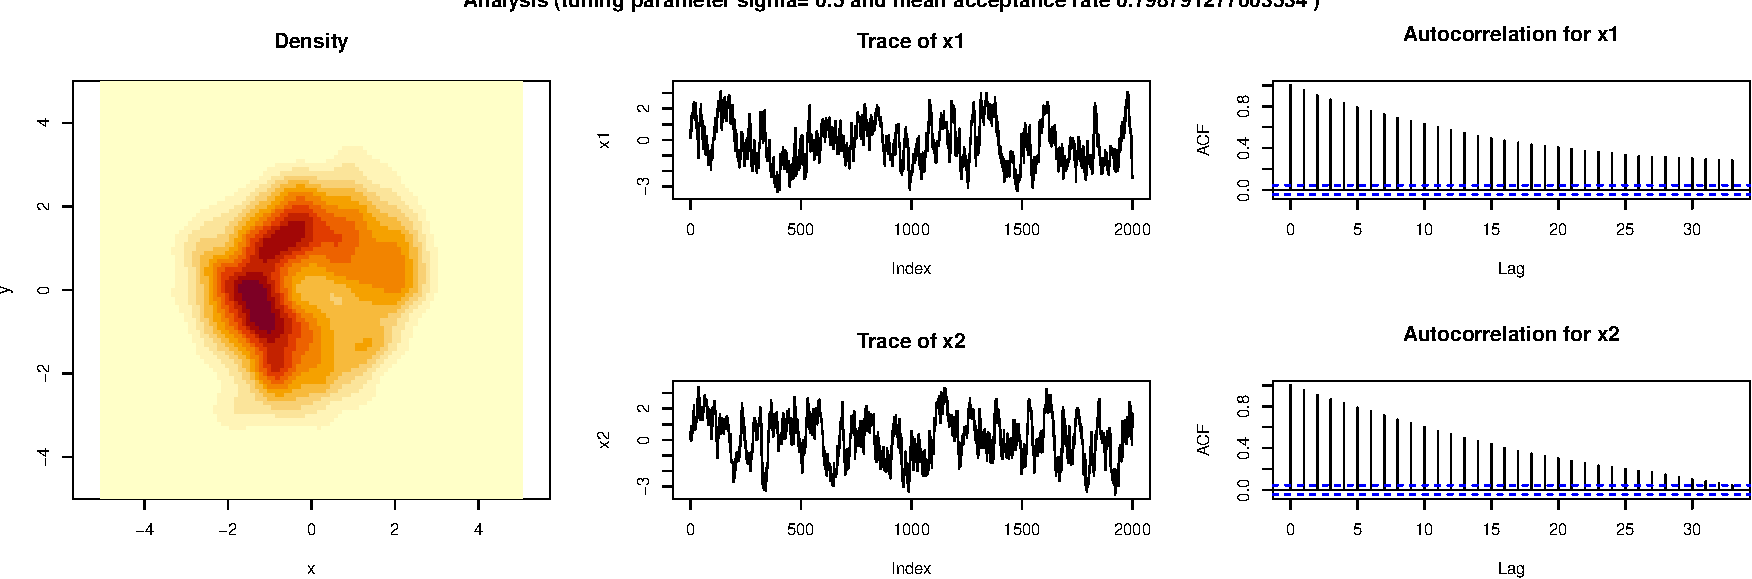
\includegraphics{Project1_files/figure-latex/RandomWalk3-2.pdf}

\begin{Shaded}
\begin{Highlighting}[]
\NormalTok{sigma =}\StringTok{ }\FloatTok{1.5}
\NormalTok{trace3 =}\StringTok{ }\KeywordTok{mcmc}\NormalTok{(x0, n, RWproposal, RWacceptance, myVolcano )}
\KeywordTok{MCMCplots}\NormalTok{(trace3)}
\end{Highlighting}
\end{Shaded}

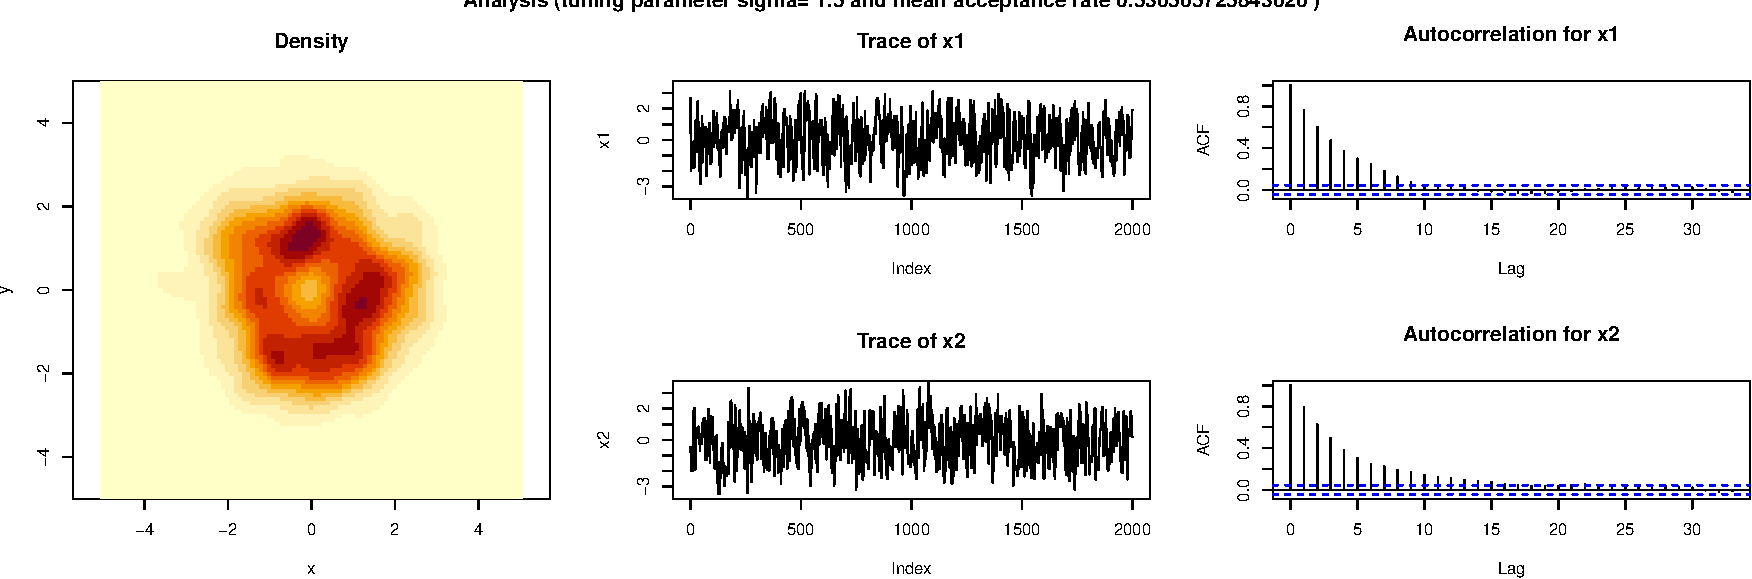
\includegraphics{Project1_files/figure-latex/RandomWalk3-3.pdf}

\begin{Shaded}
\begin{Highlighting}[]
\NormalTok{sigma =}\StringTok{ }\FloatTok{2.5}
\NormalTok{trace3 =}\StringTok{ }\KeywordTok{mcmc}\NormalTok{(x0, n, RWproposal, RWacceptance, myVolcano )}
\KeywordTok{MCMCplots}\NormalTok{(trace3)}
\end{Highlighting}
\end{Shaded}

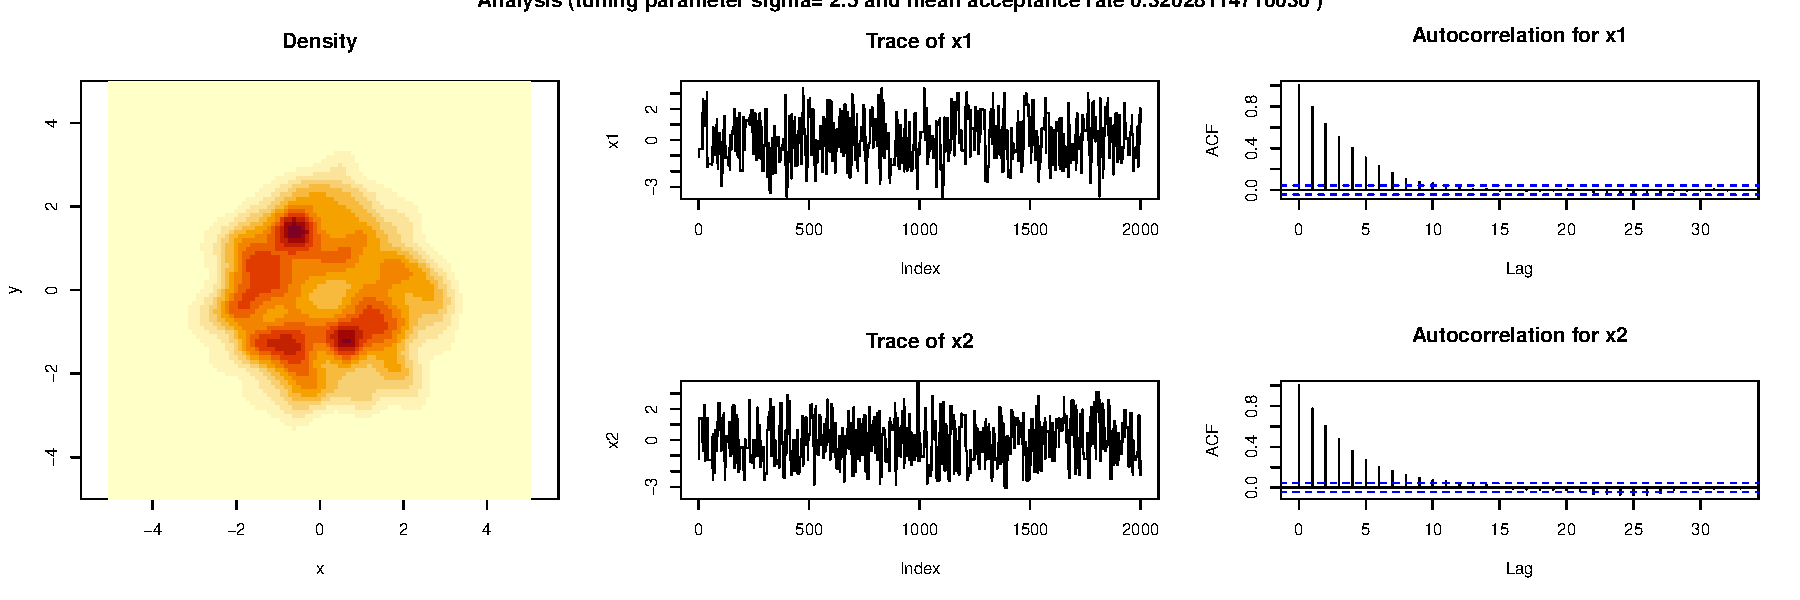
\includegraphics{Project1_files/figure-latex/RandomWalk3-4.pdf}

If the tuning parameter is chosen too small \(\sigma=0.1\) the chain
does not explore the entire ring, but get stuck. When increasing
\(\sigma\) the chain starts to walk along the circle, but for higher
parameters like \(\sigma=1.5\) the chain explores the ring with a short
autocorrelation (figuratively speaking, it can also jump from one side
toe the other and does not need to walk along the circle).

\hypertarget{conclusion}{%
\subsubsection{Conclusion}\label{conclusion}}

For all examples, there is a range of runing parameters which explore
the state-space, but the autocorrelation is still pretty high.

\hypertarget{langevin-mh}{%
\subsection{1.3 Langevin MH}\label{langevin-mh}}

Based on the Langevin dynamics and its Euler-Maruyama discretisation,
the MALA algorithm uses gradient information to define the proposal
density.

\begin{Shaded}
\begin{Highlighting}[]
\CommentTok{# Loads}
\KeywordTok{library}\NormalTok{(mvtnorm)}

\CommentTok{# Arguments:}
\CommentTok{# x_old = old state [x_1,x_2]}
\CommentTok{# dens = target density (from local variables)}

\CommentTok{# Function:}
\CommentTok{# Using 2nd order central-FD }

\CommentTok{# Return:}
\CommentTok{# Lgrad = grad (log (dens(x_old)))}
\NormalTok{Lgrad <-}\StringTok{ }\ControlFlowTok{function}\NormalTok{(x_old)\{}
\NormalTok{  Lgrad =}\StringTok{ }\KeywordTok{rep}\NormalTok{(}\DecValTok{0}\NormalTok{,}\KeywordTok{length}\NormalTok{(x_old))}
\NormalTok{  h =}\StringTok{ }\FloatTok{1e-3}
\NormalTok{  e1 =}\StringTok{ }\KeywordTok{c}\NormalTok{(}\DecValTok{1}\NormalTok{,}\DecValTok{0}\NormalTok{)}
\NormalTok{  e2 =}\StringTok{ }\KeywordTok{c}\NormalTok{(}\DecValTok{0}\NormalTok{,}\DecValTok{1}\NormalTok{)}
\NormalTok{  Lgrad[}\DecValTok{1}\NormalTok{] =}\StringTok{ }\NormalTok{(}\OperatorTok{-}\KeywordTok{log}\NormalTok{(}\KeywordTok{dens}\NormalTok{(x_old}\OperatorTok{-}\NormalTok{h}\OperatorTok{*}\NormalTok{e1)) }\OperatorTok{+}\StringTok{ }\KeywordTok{log}\NormalTok{(}\KeywordTok{dens}\NormalTok{(x_old}\OperatorTok{+}\NormalTok{h}\OperatorTok{*}\NormalTok{e1)))}\OperatorTok{/}\NormalTok{(}\DecValTok{2}\OperatorTok{*}\NormalTok{h)}
\NormalTok{  Lgrad[}\DecValTok{2}\NormalTok{] =}\StringTok{ }\NormalTok{(}\OperatorTok{-}\KeywordTok{log}\NormalTok{(}\KeywordTok{dens}\NormalTok{(x_old}\OperatorTok{-}\NormalTok{h}\OperatorTok{*}\NormalTok{e2)) }\OperatorTok{+}\StringTok{ }\KeywordTok{log}\NormalTok{(}\KeywordTok{dens}\NormalTok{(x_old}\OperatorTok{+}\NormalTok{h}\OperatorTok{*}\NormalTok{e2)))}\OperatorTok{/}\NormalTok{(}\DecValTok{2}\OperatorTok{*}\NormalTok{h)}
  \KeywordTok{return}\NormalTok{(Lgrad)}
\NormalTok{\}}

\CommentTok{# Arguments: }
\CommentTok{# x_old = old state [x_1_old, x_2_old]}

\CommentTok{# Function:}
\CommentTok{# Generating proposal following the Lnagevin MH}

\CommentTok{# Return:}
\CommentTok{# x_prop = proposed state [x_1_prop, x_2_prop]}
\NormalTok{Lproposal <-}\StringTok{ }\ControlFlowTok{function}\NormalTok{(x_old)\{}
\NormalTok{  x_prop =}\KeywordTok{c}\NormalTok{(}\KeywordTok{rmvnorm}\NormalTok{(}\DecValTok{1}\NormalTok{, x_old }\OperatorTok{+}\StringTok{ }\NormalTok{sigma}\OperatorTok{**}\DecValTok{2}\OperatorTok{/}\DecValTok{2} \OperatorTok{*}\StringTok{ }\KeywordTok{Lgrad}\NormalTok{(x_old), sigma}\OperatorTok{**}\DecValTok{2} \OperatorTok{*}\KeywordTok{diag}\NormalTok{(}\DecValTok{1}\NormalTok{,}\DecValTok{2}\NormalTok{,}\DecValTok{2}\NormalTok{))) }
  \KeywordTok{return}\NormalTok{(x_prop)}
\NormalTok{\}}

\CommentTok{# Arguments: }
\CommentTok{# x = state [x_1, x_2]}
\CommentTok{# y = condition [y_1,y_2]}

\CommentTok{# Function:}
\CommentTok{# Calculating conditional proposal density value }
\CommentTok{# for the Langevin proposal Q}

\CommentTok{# Return:}
\CommentTok{# f = Q(x|y)}
\NormalTok{dLproposal <-}\StringTok{ }\ControlFlowTok{function}\NormalTok{(x,y)\{}
\NormalTok{  f =}\StringTok{ }\KeywordTok{dmvnorm}\NormalTok{(x, y }\OperatorTok{+}\StringTok{ }\NormalTok{sigma}\OperatorTok{**}\DecValTok{2}\OperatorTok{/}\DecValTok{2} \OperatorTok{*}\StringTok{ }\KeywordTok{Lgrad}\NormalTok{(y), sigma}\OperatorTok{**}\DecValTok{2} \OperatorTok{*}\KeywordTok{diag}\NormalTok{(}\DecValTok{1}\NormalTok{,}\DecValTok{2}\NormalTok{,}\DecValTok{2}\NormalTok{))}
  \KeywordTok{return}\NormalTok{(f)}
\NormalTok{\}}


\CommentTok{# Arguments: }
\CommentTok{# x_prop = proposed state [x_1_prop, x_2_prop]}
\CommentTok{# x_old = old state [x_1_old, x_2_old]}
\CommentTok{# dens = density function of target dist}

\CommentTok{# Function:}
\CommentTok{# Calculating acceptance prob for Langevin MH}

\CommentTok{# Return:}
\CommentTok{# alpha = acceptance probability (numeric)}
\NormalTok{Lacceptance <-}\StringTok{ }\ControlFlowTok{function}\NormalTok{(x_prop, x_old, dens)\{}
\NormalTok{  alpha =}\StringTok{ }\KeywordTok{min}\NormalTok{(}\DecValTok{1}\NormalTok{, }\KeywordTok{dLproposal}\NormalTok{(x_old, x_prop)}\OperatorTok{/}\KeywordTok{dLproposal}\NormalTok{(x_prop,x_old) }\OperatorTok{*}\StringTok{ }\KeywordTok{dens}\NormalTok{(x_prop)}\OperatorTok{/}\KeywordTok{dens}\NormalTok{(x_old))}
  \KeywordTok{return}\NormalTok{(alpha)}
\NormalTok{\}}
\end{Highlighting}
\end{Shaded}

\hypertarget{standard-gaussian-1}{%
\subsubsection{Standard Gaussian}\label{standard-gaussian-1}}

We first test the Langevin MH for the Gaussian with different tuning
parameters \(\sigma\) in the proposal distribution.

\begin{Shaded}
\begin{Highlighting}[]
\CommentTok{##############################}
\CommentTok{# Testing Langevin for Gaussian}

\CommentTok{# Tuning parameters}
\NormalTok{sigma =}\StringTok{ }\FloatTok{0.25} 
\NormalTok{trace1 =}\StringTok{ }\KeywordTok{mcmc}\NormalTok{(x0, n, Lproposal, Lacceptance, myGaussian )}
\KeywordTok{MCMCplots}\NormalTok{(trace1)}

\NormalTok{sigma =}\StringTok{ }\FloatTok{0.5} 
\NormalTok{trace2 =}\StringTok{ }\KeywordTok{mcmc}\NormalTok{(x0, n, Lproposal, Lacceptance, myGaussian )}
\KeywordTok{MCMCplots}\NormalTok{(trace2)}

\NormalTok{sigma =}\StringTok{ }\FloatTok{0.75}
\NormalTok{trace3 =}\StringTok{ }\KeywordTok{mcmc}\NormalTok{(x0, n, Lproposal, Lacceptance, myGaussian )}
\KeywordTok{MCMCplots}\NormalTok{(trace3)}

\NormalTok{sigma =}\StringTok{ }\FloatTok{1.0}
\NormalTok{trace4 =}\StringTok{ }\KeywordTok{mcmc}\NormalTok{(x0, n, Lproposal, Lacceptance, myGaussian )}
\KeywordTok{MCMCplots}\NormalTok{(trace4)}
\end{Highlighting}
\end{Shaded}

Even if the mean acceptance rate for small parameters \(\sigma\leq 0.5\)
is in the asymptotically optimal range, the trace evolves to slow and
with too high correlation. For \(\sigma=0.75\) the target density is
replicated - the autocorrelation decreases and the explorance is at
least acceptable. Already for \(\sigma=1.0\) the acceptance rate is too
small and the chain pauses too long to explore the space.

\hypertarget{multimodal-1}{%
\subsubsection{Multimodal}\label{multimodal-1}}

We continue with application of the Langevin MH to the Multimodal with
different tuning parameters \(\sigma\) in the proposal distribution.

\begin{Shaded}
\begin{Highlighting}[]
\CommentTok{##############################}
\CommentTok{# Testing Langevin for Multimodal}

\CommentTok{# Tuning parameters}
\NormalTok{sigma =}\StringTok{ }\FloatTok{0.25}
\NormalTok{trace1 =}\StringTok{ }\KeywordTok{mcmc}\NormalTok{(x0, n, Lproposal, Lacceptance, myMultimodal )}
\KeywordTok{MCMCplots}\NormalTok{(trace1)}

\NormalTok{sigma =}\StringTok{ }\FloatTok{0.75}
\NormalTok{trace2 =}\StringTok{ }\KeywordTok{mcmc}\NormalTok{(x0, n, Lproposal, Lacceptance, myMultimodal )}
\KeywordTok{MCMCplots}\NormalTok{(trace2)}

\NormalTok{sigma =}\StringTok{ }\FloatTok{1.0}
\NormalTok{trace3 =}\StringTok{ }\KeywordTok{mcmc}\NormalTok{(x0, n, Lproposal, Lacceptance, myMultimodal )}
\KeywordTok{MCMCplots}\NormalTok{(trace3)}

\NormalTok{sigma =}\StringTok{ }\FloatTok{1.5}
\NormalTok{trace4 =}\StringTok{ }\KeywordTok{mcmc}\NormalTok{(x0, n, Lproposal, Lacceptance, myMultimodal )}
\KeywordTok{MCMCplots}\NormalTok{(trace4)}
\end{Highlighting}
\end{Shaded}

For small tuning parameter \(\sigma\leq 0.75\) the Langevin chain get
stuck in the local maxima of the multimodal dsitribution too long and
hence does explore the other modes too badly. For higher parameters
\(\sigma\geq1.0\) the chains reduce their autocorrelation and start to
explore all modes.

\hypertarget{volcano-1}{%
\subsubsection{Volcano}\label{volcano-1}}

Finally, we try the Langevin MH for the volcano shaped density.

\begin{Shaded}
\begin{Highlighting}[]
\CommentTok{##############################}
\CommentTok{# Testing Langevin for Multimodal}

\CommentTok{# Tuning parameters}
\NormalTok{sigma =}\StringTok{ }\FloatTok{0.25}
\NormalTok{trace1 =}\StringTok{ }\KeywordTok{mcmc}\NormalTok{(x0, n, Lproposal, Lacceptance, myVolcano )}
\KeywordTok{MCMCplots}\NormalTok{(trace1)}

\NormalTok{sigma =}\StringTok{ }\FloatTok{0.75}
\NormalTok{trace2 =}\StringTok{ }\KeywordTok{mcmc}\NormalTok{(x0, n, Lproposal, Lacceptance, myVolcano )}
\KeywordTok{MCMCplots}\NormalTok{(trace2)}

\NormalTok{sigma =}\StringTok{ }\FloatTok{1.5}
\NormalTok{trace3 =}\StringTok{ }\KeywordTok{mcmc}\NormalTok{(x0, n, Lproposal, Lacceptance, myVolcano )}
\KeywordTok{MCMCplots}\NormalTok{(trace3)}

\NormalTok{sigma =}\StringTok{ }\FloatTok{2.5}
\NormalTok{trace4 =}\StringTok{ }\KeywordTok{mcmc}\NormalTok{(x0, n, Lproposal, Lacceptance, myVolcano )}
\KeywordTok{MCMCplots}\NormalTok{(trace4)}
\end{Highlighting}
\end{Shaded}

For resonably big choices of \(\sigma=1.5\) a chain can be generated
which does explore the entire ring with small autocorrelation and an
acceptance rate close to the asymptotic optimum. For too small and too
big choices the same as for the Random Walk holds: Only a fraction of
the ring is explored for too small \(\sigma=0.25\), then the chains
starts to walk along the circle for \(\sigma=0.5\). For too big proposal
spread with \(\sigma=2.5\) too many large steps will be rejected.

\hypertarget{conclusion-1}{%
\subsubsection{Conclusion}\label{conclusion-1}}

We saw that the MALA algorithm is very sensitive to small changes in
tuning parameter \(\sigma\). For too small choices it tends to get stuck
in local maxima, what is a known issue and we realized that behaviour
here as well.

For the Gaussian distribution, the Langevin MCMC version works nicely,
but the Random Walk does not perform bad here either. In the Multimodal
case, the Random walk with suitable proposal spread does not get stuck
in a maximum as the Langevin did. The circular density without clear
mode is difficult for both MCMC versions, but the Langevin can be
parametrised to handle is better. However, in general it depends a lot
on the proper tuning for both.

\hypertarget{hamiltonian-mh}{%
\subsection{1.4 Hamiltonian MH}\label{hamiltonian-mh}}

\begin{Shaded}
\begin{Highlighting}[]
\NormalTok{K <-}\StringTok{ }\ControlFlowTok{function}\NormalTok{(p)\{ }\CommentTok{# kinetic energy is assmued to be sum(p^2/2)}
    \KeywordTok{return}\NormalTok{(}\KeywordTok{sum}\NormalTok{(}\KeywordTok{t}\NormalTok{(p) }\OperatorTok\StringTok{ }\NormalTok{p) }\OperatorTok{/}\StringTok{ }\DecValTok{2}\NormalTok{)}
\NormalTok{\}}

\NormalTok{HMC_acceptance <-}\StringTok{ }\ControlFlowTok{function}\NormalTok{(x_prop, x_old, dens)\{}
\NormalTok{    U_old <-}\StringTok{ }\OperatorTok{-}\KeywordTok{log}\NormalTok{(}\KeywordTok{dens}\NormalTok{(x_old)) }\CommentTok{# evaluate potential energy at the start of the trajectory}
\NormalTok{    U_prop <-}\StringTok{ }\OperatorTok{-}\KeywordTok{log}\NormalTok{(}\KeywordTok{dens}\NormalTok{(x_prop)) }\CommentTok{# evaluate potential energy at the end of the trajectory}
\NormalTok{    alpha =}\StringTok{ }\KeywordTok{min}\NormalTok{(}\DecValTok{1}\NormalTok{, }\KeywordTok{exp}\NormalTok{(U_old }\OperatorTok{-}\StringTok{ }\NormalTok{U_prop }\OperatorTok{+}\StringTok{ }\NormalTok{K_old }\OperatorTok{-}\StringTok{ }\NormalTok{K_prop)) }\CommentTok{# acceptance rate}
    \KeywordTok{return}\NormalTok{(alpha)}
\NormalTok{\}}

\NormalTok{HMC_proposal <-}\StringTok{ }\ControlFlowTok{function}\NormalTok{(x_old)\{}
\NormalTok{    x <-}\StringTok{ }\NormalTok{x_old}
\NormalTok{    p <-}\StringTok{ }\KeywordTok{rnorm}\NormalTok{(}\KeywordTok{length}\NormalTok{(x), }\DecValTok{0}\NormalTok{, }\DecValTok{1}\NormalTok{)}
\NormalTok{    p_old <-}\StringTok{ }\NormalTok{p}
\NormalTok{    res_leapfrog =}\StringTok{ }\KeywordTok{leapfrog}\NormalTok{(p, x, delta, L, dU)}
\NormalTok{    p =}\StringTok{ }\OperatorTok{-}\StringTok{ }\NormalTok{res_leapfrog[, }\DecValTok{1}\NormalTok{] }\CommentTok{# negate momentum at the end of trajectory to make the proposal symmetric}
\NormalTok{    x =}\StringTok{ }\NormalTok{res_leapfrog[, }\DecValTok{2}\NormalTok{] }\CommentTok{# proposed location}
\NormalTok{    K_old =}\StringTok{ }\KeywordTok{K}\NormalTok{(p_old) }\CommentTok{# evaluate kinetic energy at start of the trajectory}
\NormalTok{    K_prop =}\StringTok{ }\KeywordTok{K}\NormalTok{(p) }\CommentTok{# evaluate kinetic energy at end of the trajectory}
    \KeywordTok{return}\NormalTok{(x)}
\NormalTok{\}}

\NormalTok{leapfrog <-}\StringTok{ }\ControlFlowTok{function}\NormalTok{(p, x, delta, L, dU)\{}
\NormalTok{    p <-}\StringTok{ }\NormalTok{p }\OperatorTok{-}\StringTok{ }\NormalTok{delta }\OperatorTok{*}\StringTok{ }\KeywordTok{dU}\NormalTok{(x) }\OperatorTok{/}\StringTok{ }\DecValTok{2} \CommentTok{# make a half step for momentum at the beginning}
    \ControlFlowTok{for}\NormalTok{ (i }\ControlFlowTok{in} \DecValTok{1}\OperatorTok{:}\NormalTok{L)\{}
\NormalTok{        x <-}\StringTok{ }\NormalTok{x }\OperatorTok{+}\StringTok{ }\NormalTok{delta }\OperatorTok{*}\StringTok{ }\NormalTok{p }\CommentTok{# make a full step for the position}
        \ControlFlowTok{if}\NormalTok{ (i }\OperatorTok{!=}\StringTok{ }\NormalTok{L) p <-}\StringTok{ }\NormalTok{p }\OperatorTok{-}\StringTok{ }\NormalTok{delta }\OperatorTok{*}\StringTok{ }\KeywordTok{dU}\NormalTok{(x) }\CommentTok{# make a full step for the momentum, except at end of trajectory}
\NormalTok{    \}}
\NormalTok{    p <-}\StringTok{ }\NormalTok{p }\OperatorTok{-}\StringTok{ }\NormalTok{delta }\OperatorTok{*}\StringTok{ }\KeywordTok{dU}\NormalTok{(x) }\OperatorTok{/}\StringTok{ }\DecValTok{2} \CommentTok{# make half step for momentum at the end}
    \KeywordTok{return}\NormalTok{(}\KeywordTok{cbind}\NormalTok{(p, x))}
\NormalTok{\}}

\NormalTok{U <-}\StringTok{ }\ControlFlowTok{function}\NormalTok{(x)\{}
  \CommentTok{# U is the potential energy at given location}
    \KeywordTok{return}\NormalTok{(}\OperatorTok{-}\KeywordTok{log}\NormalTok{(}\KeywordTok{dens}\NormalTok{(x)))}
\NormalTok{\}}

\NormalTok{dU <-}\StringTok{ }\ControlFlowTok{function}\NormalTok{(x_old)\{}
  \CommentTok{# dU gives respective partial derivatives}
\NormalTok{    du =}\StringTok{ }\KeywordTok{grad}\NormalTok{(U, x_old)}
    \ControlFlowTok{if}\NormalTok{ (}\KeywordTok{any}\NormalTok{(}\KeywordTok{is.nan}\NormalTok{(du)))\{}
\NormalTok{        du =}\StringTok{ }\KeywordTok{c}\NormalTok{(}\DecValTok{0}\NormalTok{, }\DecValTok{0}\NormalTok{)}
\NormalTok{    \}}
    \KeywordTok{return}\NormalTok{(du)}
\NormalTok{\}}
\end{Highlighting}
\end{Shaded}

\begin{verbatim}




## Conclusion

- Burn-in
- All require tuning
- Compare performance



# 2 RStan

We consider the example of George et al. For a set of $N=10$ pumps we observe the values
- $y_i$: number of times that pump $i$ failed
- $t_i$: operation time of pump $i$
whose data is used as input in the next chunk.


```r
# Define list with data input
data = list(
    N=10, 
    y=c(5,1,5,14,3,19,1,1,4,22), 
    t=c(94.3,15.7,62.9,126.0,5.24,31.4,1.05,1.05,2.1,10.5)
    )
\end{verbatim}

The numbers of failures per pump are modelled by a
\(Poisson(\lambda_i t_i)\) likelihood together with a
\(Gamma(\alpha,\beta)\) distributed prior for the \(\lambda_i\) with
always \(i=1,\dots,N\). Additionally, the hyper-prior for \(\alpha\) is
\(Exp(1.0)\) and for \(\beta\) it is \(Gamma(0.1,1.0)\) respectively.
Therewith, we define a \texttt{stan} model.

NB! We do not use a separate \texttt{.stan}-file but generate the model
named ``pump'' directly in the environment. The syntax for the model
generation is exactly the same as in files, but later the function call
for the model fit deviates! The \texttt{pump.stan} file is only included
for the seek of accordance with the exercise sheet.

\begin{verbatim}
// generates a stan model named pump in the current environment

data{
  int<lower=0> N;       // number of pumps
  int<lower=0> y[N];    // number of failures
  real<lower=0> t[N];   // operation times of pumps
}

parameters{
  real<lower=0> lambda[N];
  real<lower=0> alpha;
  real<lower=0> beta;
}

transformed parameters{
  real<lower=0> eta[N];
  for (i in 1:N)
    eta[i] = lambda[i] * t[i];
}

model{
  target += exponential_lpdf( alpha | 1.0 );      // hyper-prior log-density
  target += gamma_lpdf( beta | 0.1, 1.0 );        // hyper-prior log-density
  target += gamma_lpdf( lambda | alpha, beta );   // prior log-density
  target += poisson_lpmf( y | eta );              // likelihood log-density
}
\end{verbatim}

We sample from the posterior distribution using \texttt{stan}.

NB! The function call is different since we have already a stan model
called ``pump'' in the cache and can sample from that directly.

\begin{Shaded}
\begin{Highlighting}[]
\CommentTok{# Load the RStan package}
\KeywordTok{library}\NormalTok{(rstan)}
\end{Highlighting}
\end{Shaded}

\begin{verbatim}
## Loading required package: StanHeaders
\end{verbatim}

\begin{verbatim}
## Loading required package: ggplot2
\end{verbatim}

\begin{verbatim}
## rstan (Version 2.21.2, GitRev: 2e1f913d3ca3)
\end{verbatim}

\begin{verbatim}
## For execution on a local, multicore CPU with excess RAM we recommend calling
## options(mc.cores = parallel::detectCores()).
## To avoid recompilation of unchanged Stan programs, we recommend calling
## rstan_options(auto_write = TRUE)
\end{verbatim}

\begin{Shaded}
\begin{Highlighting}[]
\CommentTok{# Fit the model using stan}
\NormalTok{fit <-}\StringTok{ }\KeywordTok{sampling}\NormalTok{(}
\NormalTok{  pump,}
  \DataTypeTok{data =}\NormalTok{ data,}
  \DataTypeTok{chains =} \DecValTok{4}\NormalTok{,}
  \DataTypeTok{warmup =} \DecValTok{1000}\NormalTok{,}
  \DataTypeTok{iter =} \DecValTok{2000}\NormalTok{,}
  \DataTypeTok{seed =} \DecValTok{1}\NormalTok{,}
  \DataTypeTok{control =} \KeywordTok{list}\NormalTok{(}\DataTypeTok{adapt_delta =} \FloatTok{0.9}\NormalTok{)}
\NormalTok{)}
\end{Highlighting}
\end{Shaded}

\begin{verbatim}
## 
## SAMPLING FOR MODEL '459e77192bc13dc921eabddda5d77169' NOW (CHAIN 1).
## Chain 1: 
## Chain 1: Gradient evaluation took 1.9e-05 seconds
## Chain 1: 1000 transitions using 10 leapfrog steps per transition would take 0.19 seconds.
## Chain 1: Adjust your expectations accordingly!
## Chain 1: 
## Chain 1: 
## Chain 1: Iteration:    1 / 2000 [  0%]  (Warmup)
## Chain 1: Iteration:  200 / 2000 [ 10%]  (Warmup)
## Chain 1: Iteration:  400 / 2000 [ 20%]  (Warmup)
## Chain 1: Iteration:  600 / 2000 [ 30%]  (Warmup)
## Chain 1: Iteration:  800 / 2000 [ 40%]  (Warmup)
## Chain 1: Iteration: 1000 / 2000 [ 50%]  (Warmup)
## Chain 1: Iteration: 1001 / 2000 [ 50%]  (Sampling)
## Chain 1: Iteration: 1200 / 2000 [ 60%]  (Sampling)
## Chain 1: Iteration: 1400 / 2000 [ 70%]  (Sampling)
## Chain 1: Iteration: 1600 / 2000 [ 80%]  (Sampling)
## Chain 1: Iteration: 1800 / 2000 [ 90%]  (Sampling)
## Chain 1: Iteration: 2000 / 2000 [100%]  (Sampling)
## Chain 1: 
## Chain 1:  Elapsed Time: 0.049371 seconds (Warm-up)
## Chain 1:                0.043448 seconds (Sampling)
## Chain 1:                0.092819 seconds (Total)
## Chain 1: 
## 
## SAMPLING FOR MODEL '459e77192bc13dc921eabddda5d77169' NOW (CHAIN 2).
## Chain 2: 
## Chain 2: Gradient evaluation took 2.6e-05 seconds
## Chain 2: 1000 transitions using 10 leapfrog steps per transition would take 0.26 seconds.
## Chain 2: Adjust your expectations accordingly!
## Chain 2: 
## Chain 2: 
## Chain 2: Iteration:    1 / 2000 [  0%]  (Warmup)
## Chain 2: Iteration:  200 / 2000 [ 10%]  (Warmup)
## Chain 2: Iteration:  400 / 2000 [ 20%]  (Warmup)
## Chain 2: Iteration:  600 / 2000 [ 30%]  (Warmup)
## Chain 2: Iteration:  800 / 2000 [ 40%]  (Warmup)
## Chain 2: Iteration: 1000 / 2000 [ 50%]  (Warmup)
## Chain 2: Iteration: 1001 / 2000 [ 50%]  (Sampling)
## Chain 2: Iteration: 1200 / 2000 [ 60%]  (Sampling)
## Chain 2: Iteration: 1400 / 2000 [ 70%]  (Sampling)
## Chain 2: Iteration: 1600 / 2000 [ 80%]  (Sampling)
## Chain 2: Iteration: 1800 / 2000 [ 90%]  (Sampling)
## Chain 2: Iteration: 2000 / 2000 [100%]  (Sampling)
## Chain 2: 
## Chain 2:  Elapsed Time: 0.043205 seconds (Warm-up)
## Chain 2:                0.035378 seconds (Sampling)
## Chain 2:                0.078583 seconds (Total)
## Chain 2: 
## 
## SAMPLING FOR MODEL '459e77192bc13dc921eabddda5d77169' NOW (CHAIN 3).
## Chain 3: 
## Chain 3: Gradient evaluation took 1e-05 seconds
## Chain 3: 1000 transitions using 10 leapfrog steps per transition would take 0.1 seconds.
## Chain 3: Adjust your expectations accordingly!
## Chain 3: 
## Chain 3: 
## Chain 3: Iteration:    1 / 2000 [  0%]  (Warmup)
## Chain 3: Iteration:  200 / 2000 [ 10%]  (Warmup)
## Chain 3: Iteration:  400 / 2000 [ 20%]  (Warmup)
## Chain 3: Iteration:  600 / 2000 [ 30%]  (Warmup)
## Chain 3: Iteration:  800 / 2000 [ 40%]  (Warmup)
## Chain 3: Iteration: 1000 / 2000 [ 50%]  (Warmup)
## Chain 3: Iteration: 1001 / 2000 [ 50%]  (Sampling)
## Chain 3: Iteration: 1200 / 2000 [ 60%]  (Sampling)
## Chain 3: Iteration: 1400 / 2000 [ 70%]  (Sampling)
## Chain 3: Iteration: 1600 / 2000 [ 80%]  (Sampling)
## Chain 3: Iteration: 1800 / 2000 [ 90%]  (Sampling)
## Chain 3: Iteration: 2000 / 2000 [100%]  (Sampling)
## Chain 3: 
## Chain 3:  Elapsed Time: 0.050613 seconds (Warm-up)
## Chain 3:                0.055562 seconds (Sampling)
## Chain 3:                0.106175 seconds (Total)
## Chain 3: 
## 
## SAMPLING FOR MODEL '459e77192bc13dc921eabddda5d77169' NOW (CHAIN 4).
## Chain 4: 
## Chain 4: Gradient evaluation took 9e-06 seconds
## Chain 4: 1000 transitions using 10 leapfrog steps per transition would take 0.09 seconds.
## Chain 4: Adjust your expectations accordingly!
## Chain 4: 
## Chain 4: 
## Chain 4: Iteration:    1 / 2000 [  0%]  (Warmup)
## Chain 4: Iteration:  200 / 2000 [ 10%]  (Warmup)
## Chain 4: Iteration:  400 / 2000 [ 20%]  (Warmup)
## Chain 4: Iteration:  600 / 2000 [ 30%]  (Warmup)
## Chain 4: Iteration:  800 / 2000 [ 40%]  (Warmup)
## Chain 4: Iteration: 1000 / 2000 [ 50%]  (Warmup)
## Chain 4: Iteration: 1001 / 2000 [ 50%]  (Sampling)
## Chain 4: Iteration: 1200 / 2000 [ 60%]  (Sampling)
## Chain 4: Iteration: 1400 / 2000 [ 70%]  (Sampling)
## Chain 4: Iteration: 1600 / 2000 [ 80%]  (Sampling)
## Chain 4: Iteration: 1800 / 2000 [ 90%]  (Sampling)
## Chain 4: Iteration: 2000 / 2000 [100%]  (Sampling)
## Chain 4: 
## Chain 4:  Elapsed Time: 0.047509 seconds (Warm-up)
## Chain 4:                0.041215 seconds (Sampling)
## Chain 4:                0.088724 seconds (Total)
## Chain 4:
\end{verbatim}

Finally, we investigate the results of the stan fit.

\begin{Shaded}
\begin{Highlighting}[]
\CommentTok{# Printing results of fit}
\KeywordTok{print}\NormalTok{(fit)}
\end{Highlighting}
\end{Shaded}

\begin{verbatim}
## Inference for Stan model: 459e77192bc13dc921eabddda5d77169.
## 4 chains, each with iter=2000; warmup=1000; thin=1; 
## post-warmup draws per chain=1000, total post-warmup draws=4000.
## 
##              mean se_mean   sd   2.5%    25%    50%    75%  97.5% n_eff Rhat
## lambda[1]    0.06    0.00 0.03   0.02   0.04   0.06   0.08   0.12  4971    1
## lambda[2]    0.10    0.00 0.08   0.01   0.04   0.08   0.14   0.32  4460    1
## lambda[3]    0.09    0.00 0.04   0.03   0.06   0.08   0.11   0.18  4804    1
## lambda[4]    0.12    0.00 0.03   0.06   0.09   0.11   0.13   0.18  4574    1
## lambda[5]    0.61    0.00 0.32   0.15   0.37   0.55   0.77   1.36  5638    1
## lambda[6]    0.61    0.00 0.13   0.37   0.51   0.60   0.70   0.90  5525    1
## lambda[7]    0.90    0.01 0.73   0.08   0.38   0.71   1.21   2.77  4980    1
## lambda[8]    0.91    0.01 0.76   0.08   0.37   0.71   1.21   2.90  5427    1
## lambda[9]    1.61    0.01 0.77   0.49   1.05   1.48   2.04   3.49  4484    1
## lambda[10]   1.99    0.01 0.42   1.27   1.68   1.95   2.25   2.90  4243    1
## alpha        0.70    0.01 0.28   0.29   0.50   0.66   0.85   1.35  2484    1
## beta         0.92    0.01 0.55   0.18   0.52   0.81   1.19   2.26  2613    1
## eta[1]       5.68    0.03 2.40   1.95   3.94   5.34   7.08  11.35  4971    1
## eta[2]       1.60    0.02 1.26   0.13   0.68   1.31   2.20   4.96  4460    1
## eta[3]       5.61    0.03 2.39   1.94   3.84   5.30   7.02  11.04  4804    1
## eta[4]      14.60    0.06 3.74   8.08  11.96  14.30  16.93  22.76  4574    1
## eta[5]       3.18    0.02 1.66   0.81   1.96   2.90   4.05   7.10  5638    1
## eta[6]      19.15    0.06 4.24  11.74  16.16  18.84  21.83  28.42  5525    1
## eta[7]       0.95    0.01 0.77   0.09   0.40   0.75   1.28   2.91  4980    1
## eta[8]       0.95    0.01 0.80   0.08   0.39   0.74   1.27   3.04  5427    1
## eta[9]       3.38    0.02 1.62   1.03   2.20   3.11   4.28   7.33  4484    1
## eta[10]     20.85    0.07 4.42  13.29  17.68  20.49  23.66  30.44  4243    1
## lp__       -43.97    0.07 2.67 -50.16 -45.53 -43.57 -42.00 -39.90  1524    1
## 
## Samples were drawn using NUTS(diag_e) at Wed Feb 17 14:15:47 2021.
## For each parameter, n_eff is a crude measure of effective sample size,
## and Rhat is the potential scale reduction factor on split chains (at 
## convergence, Rhat=1).
\end{verbatim}

\begin{Shaded}
\begin{Highlighting}[]
\CommentTok{# Plotting results of fit}
\CommentTok{# (Due to different scales we separate the plots)}
\KeywordTok{plot}\NormalTok{(fit, }\DataTypeTok{pars=}\StringTok{"lambda"}\NormalTok{)}
\end{Highlighting}
\end{Shaded}

\begin{verbatim}
## ci_level: 0.8 (80% intervals)
\end{verbatim}

\begin{verbatim}
## outer_level: 0.95 (95% intervals)
\end{verbatim}

\includegraphics{Project1_files/figure-latex/checking-1.pdf}

\begin{Shaded}
\begin{Highlighting}[]
\KeywordTok{plot}\NormalTok{(fit, }\DataTypeTok{pars=}\KeywordTok{c}\NormalTok{(}\StringTok{"alpha"}\NormalTok{, }\StringTok{"beta"}\NormalTok{))}
\end{Highlighting}
\end{Shaded}

\begin{verbatim}
## ci_level: 0.8 (80% intervals)
## outer_level: 0.95 (95% intervals)
\end{verbatim}

\includegraphics{Project1_files/figure-latex/checking-2.pdf}

\begin{Shaded}
\begin{Highlighting}[]
\KeywordTok{plot}\NormalTok{(fit, }\DataTypeTok{pars=}\StringTok{"eta"}\NormalTok{)}
\end{Highlighting}
\end{Shaded}

\begin{verbatim}
## ci_level: 0.8 (80% intervals)
## outer_level: 0.95 (95% intervals)
\end{verbatim}

\includegraphics{Project1_files/figure-latex/checking-3.pdf}

\begin{Shaded}
\begin{Highlighting}[]
\KeywordTok{traceplot}\NormalTok{(fit, }\DataTypeTok{pars=}\StringTok{"lambda"}\NormalTok{, }\DataTypeTok{inc_warmup=}\OtherTok{TRUE}\NormalTok{, }\DataTypeTok{nrow=}\DecValTok{2}\NormalTok{)}
\end{Highlighting}
\end{Shaded}

\includegraphics{Project1_files/figure-latex/checking-4.pdf}

\begin{Shaded}
\begin{Highlighting}[]
\KeywordTok{traceplot}\NormalTok{(fit, }\DataTypeTok{pars=}\KeywordTok{c}\NormalTok{(}\StringTok{"alpha"}\NormalTok{,}\StringTok{"beta"}\NormalTok{), }\DataTypeTok{inc_warmup=}\OtherTok{TRUE}\NormalTok{, }\DataTypeTok{nrow=}\DecValTok{2}\NormalTok{)}
\end{Highlighting}
\end{Shaded}

\includegraphics{Project1_files/figure-latex/checking-5.pdf}

\begin{Shaded}
\begin{Highlighting}[]
\KeywordTok{traceplot}\NormalTok{(fit, }\DataTypeTok{pars=}\StringTok{"eta"}\NormalTok{, }\DataTypeTok{inc_warmup=}\OtherTok{TRUE}\NormalTok{, }\DataTypeTok{nrow=}\DecValTok{2}\NormalTok{)}
\end{Highlighting}
\end{Shaded}

\includegraphics{Project1_files/figure-latex/checking-6.pdf}

From the print output of the fitted model, we analyse the effective
sample size \texttt{n\_eff}. With only 4.000 post-warmup draws in total,
for the \(\lambda\) (and \(\eta\)) the effective samples size is around
5.000 and thereby surprisingly higher as the actual number of samples!
In contrast for \(\alpha\) and \(\beta\), the effective sample size is
only around 2500 and 3000, respectively, such that the quality of those
samples is not as good as for the oother quantities.

In the trace plots for \(\lambda\) (and \(eta\)) we see that the state
space is explored very effectively throughout the entire chains. Maybe
for \(i\in\{5,7,9\}\) the range of lower probability is not perfectly
covered, but that is hard/impossible to say without further histograms.
In general, we can assume that the chains reached a behaviour of the
limit distribution already after a few dozen steps. For \(\alpha\) and
\(\beta\) we observe some higher autocorrelation and a less effective
exploration of the target space. For a few dozen steps the sampels
appear to remain close before the next jump comes, what is an undesired
behavior.

\end{document}
